\documentclass[11pt]{article}
\usepackage{acl}
\usepackage{times}
\usepackage{latexsym}
\usepackage[T1]{fontenc}
\usepackage[utf8]{inputenc}
\usepackage{microtype}

\usepackage{booktabs}
\usepackage{multirow}
\usepackage{amsmath}
\usepackage{amssymb}
\usepackage{graphicx}
\usepackage{tikz}
\usepackage{xcolor}
\usepackage{array}
\usepackage{makecell}
\usepackage{listings}
\usepackage{float}
\usepackage{algorithm}
\usepackage{algpseudocode}
\usetikzlibrary{arrows.meta, fit, positioning}

\hyphenpenalty=10000
\exhyphenpenalty=10000
\sloppy

\lstset{
  basicstyle=\small\ttfamily,
  breaklines=true,
  columns=flexible,
  frame=single,
  captionpos=b
}

\title{IndicNeuroSym: Neuro-Symbolic Constrained Decoding for\\
       Classical Dravidian Metrical Poetry\\
       \large Telugu \textit{Dvipada} and Kannada \textit{Ragale}}

\author{
  Samvaran K. Rallabandi, Mahesh Emani, \\ 
  {\bf Pradeep Pachipulusu}, and {\bf Faviana Noronha} \\
  IIIT Hyderabad \\
  \texttt{\small \{samvaran.rallabandi, mahesh.emani\}@research.iiit.ac.in} \\
  \texttt{\small \{saipradeep.p, faviana.noronha\}@students.iiit.ac.in} \\
}

\begin{document}
\maketitle

% -------------------------------------------------------------------------
\begin{abstract}
% -------------------------------------------------------------------------
We present IndicNeuroSym, a neuro-symbolic pipeline for generating
metrically valid classical Dravidian poetry in two metres: Telugu
\textit{dvipada} and Kannada \textit{utsaha ragale}. Both forms enforce
strict prosodic rules over syllable weight (\textit{guru}/\textit{laghu}),
metrical foot patterns (\textit{ga\d{n}a}), and second-syllable rhyme
(\textit{pr\={a}sa}); \textit{dvipada} additionally requires caesura
alliteration (\textit{yati}). We curate a validated corpus of 27,881
\textit{dvipada} couplets from five classical Telugu sources together with
1,010 synthetic Kannada \textit{ragale} poems, achieving 100\% prosodic
integrity by construction via a custom chandas scanner. We fine-tune
Gemma~3~1B with LoRA on instruction-tuned pairs and pair it with a
constrained decoder that intercepts token logits through a chained
Finite State Transducer (FST) pipeline feeding parallel Non-deterministic
Finite Automata (NFAs) for each prosodic constraint. We benchmark twelve
configurations (two models $\times$ three decoding strategies $\times$ two
languages, 1{,}224 generations total): the hybrid strategy---NFA
alive-predicate masking plus a second accept-state re-ranking pass over
the masked top-$100$---reaches \textbf{100\% poem accuracy} on both
metres with the fine-tuned model and on \textit{dvipada} even with the
base model.
LoRA fine-tuning lifts Kannada masking-only validity from 12.7\% to
96.1\%, demonstrating that adapter training collapses most of the
symbolic search burden into the model prior. As an external comparison we port the
top-$k$ constrained decoding algorithm of
Chandomitra~\citep{jagadeeshan2026chandomitra} (the closest published
constraint-decoding system for Indic metrical poetry, originally targeting
Sanskrit Anu\d{s}\d{t}ubh) to the Dvipada rule set; on the same models
and seeds the adapted port reaches 1.0\% / 13.7\% poem accuracy, against
which our hybrid achieves $7.3\times$ higher accuracy and nearly
$40\times$ lower per-poem latency on the merged model.
\end{abstract}

% -------------------------------------------------------------------------
\section{Introduction}
\label{sec:intro}
% -------------------------------------------------------------------------

Classical Telugu literature contains a rich tradition of structured poetic
forms. Among these, \textit{dvipada} (literally ``two feet'') is one of the
oldest metres, forming the backbone of major epics such as
\textit{Ranganatha Ramayanamu} (13th century) and
\textit{Basavapuranamu}. A \textit{dvipada} couplet consists of exactly two
lines (\textit{p\={a}dalu}), each composed of four metrical feet
(\textit{ga\d{n}alu}): three Indra-class feet followed by one Surya-class
foot. Additional constraints govern second-syllable consonant rhyme
(\textit{pr\={a}sa}) and alliterative harmony between designated feet within
a line (\textit{yati}).

Generating metrically valid classical poetry in these languages presents
three core challenges:
(i)~standard subword tokenizers (including the SentencePiece tokenizer
used by Gemma~3) fragment \textit{ak\d{s}aras} (syllables) across
prosodic boundaries~\citep{sennrich2016};
(ii)~the metrical constraints are tight in both traditions, with Telugu
\textit{dvipada} simultaneously enforcing \textit{ga\d{n}a},
\textit{pr\={a}sa}, and \textit{yati}, and Kannada \textit{utsaha ragale}
demanding strict \textit{pr\={a}sa}, fixed 3+3+3+\textit{guru}
\textit{ga\d{n}a} alignments, and a ban on iambic
(\textit{laghu}--\textit{guru}) sequences within any line
(\textit{p\={a}da});
and (iii)~annotated training corpora for these classical Dravidian
metrical forms are exceptionally scarce.

This paper makes four contributions: (1)~a curated, rigorously validated
corpus of 27,881 \textit{dvipada} couplets with Telugu and English
meanings, complemented by 1,010 synthetic Kannada \textit{ragale} poems
at 100\% prosodic integrity by construction; (2)~an instruction
fine-tuning (IFT) dataset and training pipeline that produces a per-language
LoRA adapter for Gemma~3~1B; (3)~a neuro-symbolic constrained decoding
architecture pairing a chained Finite State Transducer (FST) pipeline with
parallel Non-deterministic Finite Automata (NFAs), one per prosodic
constraint, that guarantees metrical validity by construction; and (4)~an
end-to-end benchmark of 1{,}224 constrained generations across twelve
configurations (two models $\times$ three decoding strategies $\times$ two
languages), plus an external head-to-head comparison on Dvipada against our port
of Chandomitra's top-$k$ constrained-decoding
algorithm~\citep{jagadeeshan2026chandomitra}, all positioned within
the Generation and Analysis taxonomy of \citet{Kranti2024}.

% -------------------------------------------------------------------------
\section{Related Work}
\label{sec:related}
% -------------------------------------------------------------------------

\paragraph{Constrained text generation.}
Constrained decoding frameworks enforce formal constraints during token
generation without model retraining. Outlines~\citep{willard2023efficient}
uses FSMs for JSON and regex constraints; LMQL~\citep{beurer2023prompting}
provides a query language for structured generation; and
Guidance~\citep{guidance} implements grammar-constrained decoding via token
masking. Our work extends this line to Telugu and Kannada prosodic metres, where constraints
derive from classical chandas treatises.

\paragraph{Multilingual sentence embeddings.}
Cross-lingual alignment is evaluated using LaBSE~\citep{feng2022languageagnostic}, while intra-lingual poem-to-meaning similarity is assessed via mSBERT~\citep{reimers2020multilingual}. To provide a specialized comparison for Indic languages, L3Cube-IndicSBERT~\citep{deode2023l3cubeindicsbertsimpleapproachlearning} is incorporated into the analysis. Furthermore, the LLM-as-a-Judge evaluation protocol is modeled after the G-Eval~\citep{liu2023geval} and GEMBA~\citep{kocmi2023gemba} metrics.

\paragraph{Computational prosody for Indic languages.}
Prior work on Indic metre analysis has focused primarily on Sanskrit;
the closest precedent is Chandomitra~\citep{jagadeeshan2026chandomitra},
a constraint-decoding system for Sanskrit Anu\d{s}\d{t}ubh poetry. At
each generation step Chandomitra's Algorithm~1 samples the top-$k$
candidate tokens, computes the resulting syllable-weight
(\textit{laghu}/\textit{guru}) sequence, and matches it against
pre-compiled \emph{fixed-length regex filters} per \textit{p\={a}da}
(e.g., \texttt{\^{}.\{4\}lgg.\$} for the first \textit{p\={a}da} of
Anu\d{s}\d{t}ubh); if no candidate matches, $k$ is widened and the
filter is re-applied. This works well on Anu\d{s}\d{t}ubh, where every
\textit{p\={a}da} is exactly eight syllables and a single fixed regex
fully specifies its valid shape (Jagadeeshan et~al.\ report 99.86\%
syntactic accuracy on Sanskrit Anu\d{s}\d{t}ubh with NLLB-distilled-1.3B
fine-tuned on their corpus). The approach does \emph{not} extend
cleanly to Telugu \textit{dvipada}, whose lines are variable-length
(11--15 syllables) and built compositionally from a vocabulary of 6+2
\textit{ga\d{n}a} patterns: expressing the legal line shape of
\textit{dvipada} requires a regular language over foot patterns rather
than a single fixed regex over syllable weights, and the metre adds
\textit{pr\={a}sa} and \textit{yati} constraints absent from
Anu\d{s}\d{t}ubh entirely. We nonetheless port Chandomitra's
Algorithm~1 to Dvipada (replacing the fixed-length per-\textit{p\={a}da}
regex with a prefix trie of all 432 valid Indra$^3$$\cdot$Surya foot
sequences and adding separate \textit{pr\={a}sa} and \textit{yati}
checks) and use it as an external baseline in
Section~\ref{sec:results}, applied to the same models, prompts, and
seeds as our enforcer. Telugu and Kannada-specific computational
prosody otherwise remains largely unexplored, and to our knowledge this
is the first study to combine formal \textit{dvipada} and
\textit{ragale} prosody rules with neural language model generation for
either language.

% -------------------------------------------------------------------------
\section{Prosodic Frameworks}
\label{sec:prosody}
% -------------------------------------------------------------------------

Both metres operate at the syllable, foot, and line levels, with rules
sourced from classical chandas treatises:
\textit{Chandhodarpanamu}~\citep{chandhodarpanamu} for Telugu
\textit{dvipada} and \citet{venkatachalashastri2008} for Kannada
\textit{utsaha ragale}. Complete rule tables appear in
Appendix~\ref{app:rules}.

\subsection{Telugu \textit{Dvipada}}
\label{sec:dvipada_prosody}

A \textit{dvipada} stanza contains exactly two lines
(\textit{p\={a}dalu}); each line comprises four metrical feet
(\textit{ga\d{n}alu}) in the fixed sequence three Indra-class feet
followed by one Surya-class foot. Each syllable is classified as heavy
(\textit{guru}, U) or light (\textit{laghu}, I): long vowels,
diphthongs, anusvara, visarga, syllable-final consonants, and the
position before a conjunct cluster yield \textit{guru}; short vowels
yield \textit{laghu} by default (full rules and the vocalic-\textit{r}
exception in Appendix~\ref{app:gurulaghu}).
Table~\ref{tab:ganas} lists the eight permitted foot patterns
(six Indra, two Surya). \textit{Pr\={a}sa} requires that the base
consonant of the second syllable of line~1 match that of line~2,
subject to three phonemic equivalence groups (laterals
$\{$la,\d{l}a$\}$, sibilants $\{$\'{s}a,sa$\}$, rhotics
$\{$\d{r}a,ra$\}$; Appendix~\ref{app:prasa}). \textit{Yati} requires
that the first syllable of foot~1 harmonically match the first
syllable of foot~3 within a line, under 11 \textit{maitri} equivalence
groups (Appendix~\ref{app:yati}). \textit{Samanya dvipada} strictly
enforces \textit{pr\={a}sa}; \textit{manjari dvipada} relaxes it.

\begin{table}[h]
\centering
\small
\caption{Permitted metrical feet (\textit{ga\d{n}alu}) for Telugu
\textit{dvipada}. U~= \textit{guru} (heavy), I~= \textit{laghu} (light).}
\label{tab:ganas}
\begin{tabular}{llll}
\toprule
\textbf{Foot} & \textbf{Pattern} & \textbf{Class} & \textbf{Beats} \\
\midrule
nala      & I\,I\,I\,I & Indra & 4 \\
naga      & I\,I\,I\,U & Indra & 5 \\
sala      & I\,I\,U\,I & Indra & 5 \\
bha       & U\,I\,I    & Indra & 4 \\
ra        & U\,I\,U    & Indra & 5 \\
ta        & U\,U\,I    & Indra & 5 \\
\midrule
na        & I\,I\,I    & Surya & 3 \\
ha / gala & U\,I       & Surya & 3 \\
\bottomrule
\end{tabular}
\end{table}

\subsection{Kannada \textit{Utsaha Ragale}}
\label{sec:utsaha_prosody}

A \textit{utsaha ragale} stanza contains two lines, each comprising
four metrical feet of exactly three syllables, yielding 12 syllables
per line. Syllable weight follows the same broad rules as Dvipada
(long vowels, diphthongs, anusvara, visarga, halant endings, and
position before a conjunct cluster all promote to \textit{guru}); the
character sets differ only in script. Word boundaries block the
conjunct rule. Table~\ref{tab:utsaha_ganas} lists the two permitted
foot patterns: III at positions~1--3 and IIU at all four positions.
The metre prohibits two-syllable patterns to preserve the triple-syllable
rhythm, and requires both lines to end on \textit{guru}, structurally
enforced by constraining position~4 to IIU. \textit{\={A}di
Pr\={a}sa} requires matching the base consonant of the second syllable
across lines (ignoring vowel marks, conjunct extensions, anusvara, and
visarga); relaxed evaluation allows two equivalence groups, laterals
$\{$la,\d{l}a$\}$ and sibilants $\{$\'{s}a,\d{s}a,sa$\}$
(Appendix~\ref{app:prasa}).

\begin{table}[h]
\centering
\small
\caption{Permitted metrical feet (\textit{ga\d{n}alu}) for Kannada
\textit{utsaha ragale}. U~= \textit{guru} (heavy), I~= \textit{laghu} (light).}
\label{tab:utsaha_ganas}
\begin{tabular}{lllr}
\toprule
\textbf{Pattern} & \textbf{Syllables} & \textbf{Allowed Positions} & \textbf{Beats} \\
\midrule
I\,I\,I & 3 & 1, 2, 3    & 3 \\
I\,I\,U & 3 & 1, 2, 3, 4 & 4 \\
\bottomrule
\end{tabular}
\end{table}

% -------------------------------------------------------------------------
\section{Dataset Construction}
\label{sec:dataset}
% -------------------------------------------------------------------------

\subsection{Sources and Curation}

To enable instruction-tuned generation in a metre with no public training
corpus, we assemble a validated \textit{dvipada} dataset from five classical
Telugu sources and complement it with 1,010 synthetic Kannada
\textit{ragale} poems across 100 topics, generated with Gemini~3~Pro to
mitigate data scarcity. Every candidate is filtered through a chandas
analyzer so that the training distribution is 100\% prosodically valid by
construction. Table~\ref{tab:sources} reports raw couplet counts, the
number passing strict 100\% prosodic compliance (\textit{pure}), and purity
rates per source.

All candidates were filtered by the Dvipada and Ragale chandas analyzers,
which verify full prosodic compliance and reject any couplet that fails
\textit{ga\d{n}a}, \textit{pr\={a}sa}, or \textit{yati}. The high
rejection rate for \textit{Palanati Vira Charitra} (91.7\%) reflects its
use of the \textit{manjari} variant, which relaxes \textit{pr\={a}sa}.
The final Telugu dataset comprises 27,881 couplets in JSON format, each
paired with a Telugu prose meaning and an English translation. The
Kannada \textit{ragale} corpus follows the same schema.

\begin{table}[h!]
\centering
\small
\resizebox{\columnwidth}{!}{% % Starts scaling
\begin{tabular}{lrrr}
\toprule
\textbf{Source} & \textbf{Raw Couplets} & \textbf{Master (Validated)} & \textbf{Purity} \\
\midrule
Ranganatha Ramayanamu  & 26,296 & 21,828 & 83.0\% \\
Basavapuranamu         &  2,454 &  1,859 & 75.8\% \\
Dvipada Bhagavatamu    &  3,157 &  2,002 & 63.4\% \\
Palanati Vira Charitra &    783 &     65 &  8.3\% \\
Srirama Parinayamu     &    392 &    374 & 95.4\% \\
Synthetic (Gemini)     &  3,496 &  1,753 & 50.1\% \\
\midrule
\textbf{Total} & \textbf{36,578} & \textbf{27,881} & \textbf{76.2\%} \\
\bottomrule
\end{tabular}% % Ends scaling
}
\caption{Dataset sources with raw couplet counts, master validated counts, and prosodic purity rates.}
\label{tab:sources}
\end{table}

\subsection{Dataset Composition}

The Telugu corpus is 93.7\% classical material (26,128 couplets) and 6.3\% synthetic
(1,753 couplets). Topics span theology, mythology, and devotional poetry,
primarily in archaic Telugu register with colloquial augmentations in the
synthetic subset. The Kannada \textit{ragale} corpus is 100\% synthetic, covering 100 topics across generic topics.
% -------------------------------------------------------------------------
\section{Data Validation}
\label{sec:validation}
% -------------------------------------------------------------------------

We certify the 27,881-couplet corpus with a five-level pipeline that
ascends from hard structural gates (Levels~1--2: prosody, prose-verse
alignment) through diagnostic semantic and lexical checks
(Levels~3--4) to a qualitative LLM-judge (Level~5); each level catches
what the previous one cannot. Table~\ref{tab:validation} summarises
pass rates.

\subsection{Level 1: Prosodic Integrity}

The chandas scanner serves as the inclusion criterion described in
Section~\ref{sec:dataset}, so the trivially necessary first check is
that every retained couplet passes it: $100\%$ ($27{,}881/27{,}881$).
This is by construction, but it pins the lower bound for everything
that follows.

\subsection{Level 2: Length Ratio Check}

A poem can be metrically valid yet paired with a prose meaning that is
either too terse or too verbose to be a faithful gloss. We enforce
$0.8 \leq |P|/|V| \leq 2.5$ (Telugu prose~$P$ over verse~$V$),
which $99.1\%$ of records pass ($27{,}633/27{,}881$). The bulk
($88.9\%$) sits in the 1.0--2.0 band; only $248$ records ($0.9\%$)
fall outside, with the five most extreme ratios at 5.11, 4.73, 4.71,
4.65, and 4.36, all suspect translations rather than valid couplets.

\subsection{Level 3: Semantic Fidelity}

Levels~1--2 check structure but not meaning, so we next quantify
semantic agreement using three multilingual sentence-embedding models,
computed on the augmented dataset ($n=29{,}343$) prior to final purity
filtering. The primary gate is LaBSE Telugu-to-English meaning
similarity $\geq 0.65$~\citep{feng2022languageagnostic}, which $77.1\%$
of pairs clear (mean 0.721), confirming that prose annotations are
translation-consistent. The other two scores
(mSBERT-mpnet~\citep{reimers2020multilingual} at $63.7\%$ on
poem-to-Telugu, L3Cube-IndicSBERT~\citep{deode2023l3cubeindicsbertsimpleapproachlearning}
at $40.1\%$) are intentionally diagnostic rather than gating: classical
\textit{dvipada} uses compressed, elliptical \textit{sam\={a}sa}
compounds that diverge structurally from modern prose paraphrases, so
low poem-to-meaning similarities are expected and reflect genre
distance, not annotation noise. The full per-pair table is in
Appendix~\ref{app:validation}.

\subsection{Level 4: Lexical Diversity}

Even with structure and meaning verified, the corpus could still be
formulaic. Level~4 therefore characterises its literary register. The
Gemma~3 tokenizer covers $74.4\%$ of the model's Telugu vocabulary
($1{,}328/1{,}784$ tokens) on $804{,}671$ corpus tokens. At the word
level, corpus TTR is $0.491$ and MATTR is $0.501$, below the
$0.70$--$0.80$ range typical of modern prose, consistent with the
formulaic repetition inherent to metrical verse. Yule's $K=3.50$ places
the corpus firmly in the literary range ($K<100$), while Honoré's
$H=6{,}165$ far exceeds the $1{,}000$--$2{,}000$ literary baseline,
indicating exceptional vocabulary richness. The hapax ratio
($V_1/V=0.804$) confirms that most word types occur exactly once. No
exact duplicates were found; $160$~poems in $79$~groups are
near-duplicates under normalisation. Full per-poem and corpus tables
are in Table~\ref{tab:lexical-diversity}, Appendix~\ref{app:validation}.

\subsection{Level 5: LLM-as-a-Judge Evaluation}

The first four levels are automatic and rule-based. Level~5 layers a
qualitative judgement on top by sampling 250 couplets stratified across
all sources and scoring them with Gemini~3~Pro (Vertex~AI Batch~API)
on a 1--5 rubric covering semantic fidelity, completeness, cultural
accuracy, and linguistic quality in Telugu and English (modelled on
G-Eval~\citep{liu2023geval} and GEMBA~\citep{kocmi2023gemba}). The
mean total is \textbf{24.25/25 ($97.0\%$)}, with per-dimension means
ranging from $4.73$ (semantic fidelity) to $4.98$ (Telugu linguistic
quality); $90.4\%$ of samples receive an overall verdict of
``Excellent'' ($226/250$), $6.4\%$ ``Good'', $2.8\%$ ``Acceptable'',
and $0.4\%$ ``Poor'' (1 sample). The per-dimension breakdown, aggregate distribution, and
source-stratification appear in Appendix~\ref{app:validation}. The five
levels combined certify a corpus that is structurally correct,
prose-verse aligned, semantically consistent, lexically rich, and
qualitatively highly rated.

\begin{table}[t]
\centering
\small
\caption{Cross-level validation summary.}
\label{tab:validation}
\begin{tabular}{llr}
\toprule
\textbf{Level} & \textbf{Description} & \textbf{Pass Rate} \\
\midrule
1 & Prosodic integrity (chandas)      & 100.0\% \\
2 & Length ratio ($0.8$--$2.5$)       &  99.1\% \\
3 & LaBSE semantic fidelity           &  77.1\% \\
4 & Lexical diversity (TTR)           & 0.90 avg \\
5 & LLM-as-a-Judge ($n{=}250$)        &  97.0\% \\
\midrule
\multicolumn{2}{l}{Pass all levels 1--3} & 68.9\% \\
\bottomrule
\end{tabular}
\end{table}

% -------------------------------------------------------------------------
\section{Fine-Tuning Dataset Preparation}
\label{sec:finetuning}
% -------------------------------------------------------------------------

The validated 27,881-entry corpus is transformed into instruction-completion
pairs for supervised fine-tuning (SFT) of Gemma~3~1B~\citep{gemma2024}
using LoRA~\citep{hu2022lora}.

\paragraph{Instruction templates.}
Each sample is assigned one instruction type from four categories:
(1)~\textbf{Generic} (``Write a Telugu \textit{dvipada} couplet following
the above rules''), available for all samples;
(2)~\textbf{Work-style} (``Compose a \textit{dvipada} in the style of
[source]''), available for non-synthetic sources;
(3)~\textbf{Meaning-conditioned (Telugu)}: ``Write a \textit{dvipada}
expressing: \{Telugu meaning\}''; and
(4)~\textbf{Meaning-conditioned (English)}: ``Write a \textit{dvipada}
expressing: \{English meaning\}''.
This diversity trains the model to respond to varied prompt styles in both
languages.

\paragraph{Rules injection.}
Every training sample's input is prefixed with the complete \textit{dvipada}
prosodic specification, covering all \textit{ga\d{n}a} patterns,
\textit{guru}/\textit{laghu} rules, \textit{pr\={a}sa}, and \textit{yati}.
This ensures the model has the metrical specification in context during both
training and inference.

\paragraph{Dataset splits.}
The pipeline produces \texttt{train.jsonl} (80\%), \texttt{val.jsonl} (10\%),
and \texttt{test.jsonl} (10\%, held out).

\subsection{Training Setup}
\label{sec:training_setup}

Table~\ref{tab:training-config} reports the LoRA fine-tuning configuration
used to produce the Dvipada merged model and the Ragale adapter benchmarked
in Section~\ref{sec:results}. Both runs share the same base model
(\texttt{google/gemma-3-1b-it}), optimizer (fused AdamW), schedule
(cosine with warmup), precision (bf16), attention backend (SDPA),
gradient checkpointing, and effective batch size~16 (via gradient
accumulation), and both target every linear projection
(\texttt{q,k,v,o,gate,up,down}) with $\textsc{bias}{=}\textsc{none}$
and dropout~$0.05$. They diverge on LoRA capacity, learning rate, warmup,
and sequence length, reflecting the $\sim$28$\times$ asymmetry between
the Telugu and Kannada training corpora (27{,}881 vs.\ 1{,}010
examples).

\begin{table}[t]
\centering
\small
\caption{LoRA fine-tuning configuration for the Dvipada merged model
and the Ragale adapter. ``All linear'' denotes
\texttt{q,k,v,o,gate,up,down} projection layers.}
\label{tab:training-config}
\resizebox{\columnwidth}{!}{%
\begin{tabular}{lll}
\toprule
\textbf{Hyperparameter} & \textbf{Telugu Dvipada} & \textbf{Kannada Ragale} \\
\midrule
Base model           & \texttt{gemma-3-1b-it} & \texttt{gemma-3-1b-it} \\
LoRA rank $r$        & \textbf{16}            & \textbf{32}            \\
LoRA $\alpha$        & 32                     & 64                     \\
LoRA dropout         & 0.05                   & 0.05                   \\
Target modules       & all linear             & all linear             \\
LoRA bias            & none                   & none                   \\
\midrule
Optimizer            & AdamW (fused)          & AdamW (fused)          \\
Learning rate        & \textbf{2e--4}         & \textbf{5e--5}         \\
LR schedule          & cosine                 & cosine                 \\
Warmup ratio         & 0.03                   & 0.06                   \\
Weight decay         & 0.01                   & 0.01                   \\
Max grad.\ norm      & 1.0                    & 1.0                    \\
\midrule
Per-device batch     & 1                      & 2                      \\
Grad.\ accum.\ steps & 16                     & 8                      \\
Effective batch      & 16                     & 16                     \\
Max seq.\ length     & 384                    & 512                    \\
Seq.\ packing        & yes                    & yes                    \\
\midrule
Epochs               & \textbf{8}             & \textbf{6}             \\
Train / val split    & 90 / 10                & 90 / 10                \\
Best-ckpt criterion  & min eval\_loss         & min eval\_loss         \\
Eval / save every    & 500 steps              & 500 steps              \\
\midrule
Precision            & bf16 + TF32            & bf16                   \\
Attention            & SDPA                   & SDPA                   \\
Grad.\ checkpointing & yes                    & yes                    \\
Hardware             & RTX 5050 (8\,GB)       & RTX 5050 (8\,GB)       \\
Seed                 & 42                     & 42                     \\
\bottomrule
\end{tabular}%
}
\end{table}

\paragraph{Why the configurations differ.}
Three asymmetries are deliberate. First, the Kannada run uses a larger
LoRA ($r{=}32$ vs.\ $r{=}16$) and a smaller learning rate
($5\text{e--}5$ vs.\ $2\text{e--}4$) to extract a useful signal from
the $\sim$1k-example Ragale corpus without overfitting; the higher
warmup ratio ($0.06$) softens the early-step gradients on the same
small data. Second, Ragale's longer max sequence length (512 vs.\ 384)
accommodates its 12-syllable-per-line structure, which produces
slightly longer instruction prompts than Dvipada's 11--15 syllable
variable-length lines. Third, both runs save the best checkpoint by
\texttt{eval\_loss}; the Dvipada adapter is then merged back into the
base weights to produce the \texttt{gemma3-1b-merged} model used in
Section~\ref{sec:results}, while the Ragale adapter is retained as a
PEFT layer on top of the base model (\texttt{gemma3-1b-lora}). This
explains the model-naming convention used in
Tables~\ref{tab:dvipada-results} and~\ref{tab:ragale-results}.

% -------------------------------------------------------------------------
\section{Constrained Decoding Architecture}
\label{sec:constrained}
% -------------------------------------------------------------------------

To provide formal metrical guarantees beyond what fine-tuning alone achieves,
we design a constrained decoding system that intercepts Gemma's token
generation and masks out any token violating \textit{dvipada} metre.

\subsection{Theoretical Basis}

Every \textit{dvipada} constraint operates on fixed positions with finite
alphabets, so the combined constraint language is regular: the
\textit{ga\d{n}a} pattern is a finite union of concatenations of finite
strings over $\{$U,I$\}$ (no stack required); \textit{pr\={a}sa} is a
single comparison at a fixed position against $\sim$30 stored consonant
classes; \textit{yati} is a single comparison at a fixed position against
11 \textit{maitri} groups. Closure of regular languages under intersection
keeps the combined machine an NFA of bounded size.


\subsection{System Overview}

At each generation step, raw logits from Gemma~3~1B pass through the
Symbolic Enforcer (Figure~\ref{fig:enforcer}, Appendix~\ref{app:fst})
before sampling. The Enforcer routes candidate tokens through a chained
FST pipeline into three parallel NFAs and emits a boolean mask
($-\infty$ for invalid tokens). The decoder strategies described below
in Section~\ref{sec:constrained_loop} consume this mask in three
different ways (Figure~\ref{fig:strategies}, Appendix~\ref{app:algorithms}).

\subsection{Layer 1: Orchestrator FST Pipeline}
\label{sec:fst}

Two chained Mealy FSTs transform raw Unicode token strings into a
classified U/I syllable stream. A stateless character classifier precedes them.

\paragraph{Stage 0: Codepoint Classifier (stateless).}
A stateless classification function classifies each Unicode codepoint into 11 categories
via an $O(1)$ set-membership check. Categories cover consonants
(U+0C15--U+0C39), independent vowels (U+0C05--U+0C14), matras
(U+0C3E--U+0C4C), virama (U+0C4D), anusvara (U+0C02), visarga (U+0C03),
ai-length mark (U+0C56), space, newline, ZWNJ, and other. This function is inlined into the Syllable Assembler rather than implemented as a separate transducer.

\paragraph{Stage 1: Syllable Assembler (4 states).}
Groups the category stream into complete Telugu syllables using states
\textsc{idle}, \textsc{consonant\_cluster}, \textsc{pending\_virama}, and
\textsc{vowel}. A one-slot \textit{prev\_syllable} buffer enables retroactive
pollu (syllable-final consonant) merging. The \textsc{pending\_virama} state
distinguishes conjunct consonants from pollu marks via lookahead.

\paragraph{Stage 2: Guru/Laghu Classifier (2 states).}
Classifies each syllable as U or I using five phonological rules from
\textit{Chandhodarpanamu}~\citep{chandhodarpanamu}, via states
\textsc{empty} and \textsc{pending\_i}. A one-syllable delay buffer in \textsc{pending\_i} enables Rule~5 (conjunct-induced weight promotion),
which applies within words but is blocked by intervening spaces.

\subsection{Layer 2: Position Tracker and Parallel NFAs}
\label{sec:nfas}

The Position Tracker routes syllable metadata to three NFAs based on the
current position within the couplet: line index (1 or 2), syllable index within the line, and line completion count.

\paragraph{Ga\d{n}a NFA ($\sim$69 states).}
Validates each line against the regular pattern
$(nala \mid naga \mid sala \mid bha \mid ra \mid ta)^3 \cdot (na \mid ha)$
over $\{$U, I$\}$. The NFA branches non-deterministically after each
syllable. Each branch is a tuple (\texttt{slot}, \texttt{gana\_name}, \texttt{sub\_pos}, \texttt{matched\_ganas}), where slot indexes the current foot (0--2 for Indra \textit{ga\d{n}as}, 3 for the Surya \textit{ga\d{n}a}). Valid line lengths range from 11 to 15 syllables.

\paragraph{Pr\={a}sa NFA (7 states).}
Phase~1 records the base consonant of the second syllable of
line~1. Phase~2 verifies that the second syllable of line~2 has a matching base consonant (checked via equivalence lookup); a mismatch transitions to the \textsc{reject} state. The 7 states are: \textsc{line1\_syl0}, \textsc{line1\_syl1}, \textsc{line1\_rest}, \textsc{line2\_syl0}, \textsc{line2\_syl1}, \textsc{accept}, and \textsc{reject}. Consonant identity is stored as a data variable, not encoded in NFA states. Three equivalence pairs (laterals: l/L, sibilants: sh/Sh/s, rhotics: R/r) are checked via lookup.

\paragraph{Yati NFA (4 states).}
The state \textsc{idle} records the phonetic information of the first syllable of \textit{ga\d{n}a}~1; \textsc{recorded} passes through \textit{ga\d{n}a}~2 silently; on entering \textit{ga\d{n}a}~3 the NFA verifies that its first syllable belongs to the same phonetic class via a 5-level cascade (exact match, \textit{vyanjana yati}, \textit{svara yati}, \textit{samyukta yati}, \textit{bindu yati}), transitioning to \textsc{accepted} on success or \textsc{rejected} on failure. Phonetic group membership (across 11 \textit{Yati Maitri} groups) is computed on demand rather than encoded in NFA states. \textit{Yati} enforcement is optional; it can be disabled
for \textit{manjari} variant generation.

\subsection{Dead State Detection}

To maintain metrical integrity, we define a \textit{Dead State Detection} mechanism. Let $\mathcal{B}$ be the set of active NFA branches. For each branch $b \in \mathcal{B}$ at state $s = (\texttt{slot}, \texttt{gana}, \texttt{pos})$, let $C(b)$ be the current syllable count. We define two closed-form heuristic functions:
\begin{itemize}
    \item $min\_dist(s)$: Minimum syllables to reach \textsc{accept} from $s$.
    \item $max\_dist(s)$: Maximum syllables to reach \textsc{accept} from $s$.
\end{itemize}

A branch $b$ is considered \textbf{viable} if it satisfies the window constraint $[L_{min}, L_{max}]$, where $L_{min}=11$ and $L_{max}=15$:
\begin{equation}
    (C(b) + \textit{min\_dist}(s) \le 15) \land (C(b) + \textit{max\_dist}(s) \ge 11)
\end{equation}

If the set of viable branches is $\emptyset$, the configuration is flagged as a \textit{dead state}, triggering immediate token pruning.

\subsection{State Budget and Design Rationale}

Using three independent NFAs achieves a $24\times$ state reduction
($69 \times 7 \times 4 = 1{,}932$ product DFA states versus $\sim$80
total separately), while enabling partial scoring, selective constraint
enforcement, and independent debugging. Per-component state counts
appear in Table~\ref{tab:states}, Appendix~\ref{app:fst}.

\subsection{Constrained Decoding Loop}
\label{sec:constrained_loop}

All three decoding strategies we benchmark rely on per-step NFA
rejection: at every generation step,
\textsc{BuildGanaMask}~(Alg.~\ref{alg:build-mask}) clones the
incremental \textsc{CompositeState}, feeds each of the $\sim$1{,}822
Telugu tokens, flushes, and keeps only those whose
\textsc{is\_alive()} predicate still holds---i.e., the token keeps the
Ga\d{n}a, Pr\=asa, and Yati NFAs jointly satisfiable. What
distinguishes the strategies is (a)~whether a recovery mechanism runs
when the alive set collapses, and (b)~whether the surviving candidates
are further re-ranked by a line-completion (\textsc{has\_accept})
preference. Full pseudocode is in Appendix~\ref{app:algorithms}; for
completeness the appendix also presents a stateless \emph{Rejection
Sampling} variant (Alg.~\ref{alg:rejection-sampling}) that runs
\textsc{AnalyzeText} on the full text per candidate and enforces only
ga\d{n}a reachability, included as an illustrative alternative but not
benchmarked in Section~\ref{sec:results}.

\textbf{Strategy~1 (Masking-Only):} a static mask first reduces the
$\sim$256K vocabulary to $\sim$1{,}822 Telugu tokens, then
\textsc{BuildGanaMask} keeps only those tokens whose
\textsc{is\_alive()} predicate holds; top-$p$ sampling runs over this
NFA-filtered set. No recovery, no accept-state re-ranking.

\textbf{Strategy~2 (Masking + Backtracking,
Alg.~\ref{alg:masking-backtrack}):} same NFA alive-predicate filtering
as Strategy~1, plus a recovery mechanism---if the alive set drops below
3 candidates or the line overshoots 15 syllables, the decoder
restores a checkpoint (ring buffer of 15 entries, saved every 3 tokens)
and escalates the sampling temperature by $+0.15$ (cap $1.2$, decay
over 6 steps).

\textbf{Strategy~3 (Hybrid Mask + Accept Preference,
Alg.~\ref{alg:hybrid}):} same NFA alive-predicate filtering as
Strategy~1, plus a \emph{second} NFA pass over the top-$100$ tokens of
the masked distribution that additionally checks
\textsc{has\_accept()} per candidate and prefers tokens that would
complete a valid line when weighted-sampling the next token.
Checkpoint backtracking is retained as a last-resort fallback but
rarely fires in practice (Section~\ref{sec:results}). The ``rejection''
in our original name for this strategy refers specifically to this
second \textsc{has\_accept} re-ranking pass, not to the underlying
alive-predicate filtering that all three strategies share.

% -------------------------------------------------------------------------
\subsection{Ragale Adaptation}
\label{sec:ragale_decoding}

For Kannada \textit{utsaha ragale} we apply the same Symbolic Enforcer
architecture with three structural simplifications driven by the rule
set of \citet{venkatachalashastri2008}: (i)~the Ga\d{n}a NFA shrinks
from 69 to 22 states, since only two foot patterns (III and IIU) are
permitted at fixed 12 syllables per line; (ii)~the Yati NFA is removed
entirely (\textit{ragale} has no caesura constraint); and (iii)~the
Pr\=asa NFA uses two Kannada-specific equivalence groups instead of
three (the Telugu rhotic group is absent). The total state budget falls
from $\sim$80 to $\sim$35; the product DFA falls from $1{,}932$ to
$154$ ($12.5\times$ smaller). All three decoding strategies apply to
Ragale without algorithmic modification, only with the reduced
\textit{ga\d{n}a} pool and the disabled yati check. Full
construction details, the Dvipada-vs-Ragale comparison table, the
Ragale state budget, and the architecture figure appear in
Appendix~\ref{app:ragale_construction}.

% -------------------------------------------------------------------------
\section{End-to-End Evaluation}
\label{sec:evaluation}
% -------------------------------------------------------------------------

We evaluate the symbolic enforcer end-to-end on both metres by running
every combination of two models and three decoding strategies for
twelve benchmark configurations. For each language we test the base
instruction-tuned model (\texttt{google/gemma-3-1b-it}) and its LoRA
fine-tuned variant (merged for Telugu, adapter for Kannada; full
hyperparameters in Section~\ref{sec:training_setup},
Table~\ref{tab:training-config}) under the three decoding strategies of
Section~\ref{sec:constrained}: \textit{masking only},
\textit{masking with checkpoint backtracking}, and the \textit{hybrid}
mask + accept-state re-ranking sampler. Each (model, method) cell generates 102
poems from 3 prompts $\times$ 34 seeds ($42 + 7k$ for $k\in[0,33]$),
giving \textbf{1{,}224 generations} across the matrix. Sampling uses
$\tau=0.7$, top-$p=0.9$, $\texttt{max\_new\_tokens}=150$, on a single
NVIDIA RTX~5050 laptop GPU with bfloat16 (no quantisation). Telugu
prompts are mythological/devotional themes drawn from the corpus
(\textit{tallI prEma annintikaMTe goppadi},
\textit{hanumaMtuDu samudramunu dATi laMkanu cErenu},
\textit{SrIrAmuDu sItAdEvini rakshiMcuTaku laMkaku veLLenu});
Kannada prompts are short topical themes (\textit{Bubbles},
\textit{Moon}, \textit{Rain}). We report \textit{poem accuracy} (fraction
of generations whose both lines pass the FST+NFA validator),
\textit{line accuracy}, mean wall time per poem, mean tokens generated,
and mean backtrack count; validation uses the same chandas pipeline
that filtered the training corpus. All twelve benchmark scripts and
result JSONs are distributed under
\texttt{domino/}\allowbreak{} (Telugu) and
\texttt{ragale\_pipeline/}\allowbreak\texttt{ragale\_\allowbreak inference\_\allowbreak scripts/}
(Kannada) in the project repository.

% -------------------------------------------------------------------------
\section{Results}
\label{sec:results}
% -------------------------------------------------------------------------

Tables~\ref{tab:dvipada-results} and~\ref{tab:ragale-results} report
poem-level accuracy for the twelve configurations. Per-topic breakdowns and
efficiency statistics are deferred to
Appendix~\ref{app:detailed_results}.

\begin{table}[t]
\centering
\small
\caption{Dvipada end-to-end constrained decoding results
($n=102$ poems per row; 3 prompts $\times$ 34 seeds). The
\textit{adapted Chandomitra} rows are our port of the
Algorithm~1 of~\citet{jagadeeshan2026chandomitra} (originally designed
for Sanskrit Anu\d{s}\d{t}ubh, 99.86\% on its native task) to the
Dvipada rule set, applied to the same models, prompts, and seeds.
All three FST+NFA strategies share the same per-step NFA
alive-predicate filter; they differ only in recovery (backtracking)
and accept-state re-ranking (hybrid).}
\label{tab:dvipada-results}
\resizebox{\columnwidth}{!}{%
\begin{tabular}{llrrrr}
\toprule
\textbf{Model} & \textbf{Method} & \textbf{Valid} &
  \textbf{Poem \%} & \textbf{Line \%} & \textbf{s/poem} \\
\midrule
\multicolumn{6}{l}{\textit{Adapted Chandomitra baseline~\citep{jagadeeshan2026chandomitra}}} \\
gemma3-1b-base   & chandomitra        &   1/102 &   1.0 &   3.4 & 37.24 \\
gemma3-1b-merged & chandomitra        &  14/102 &  13.7 &  18.1 & 58.87 \\
\midrule
\multicolumn{6}{l}{\textit{FST+NFA Symbolic Enforcer (this work)}} \\
gemma3-1b-base   & masking\_only      &  32/102 &  31.4 &  61.8 & 3.49 \\
gemma3-1b-base   & masking\_backtrack &  93/102 &  91.2 &  95.6 & 3.45 \\
gemma3-1b-base   & hybrid             & 102/102 & \textbf{100.0} & 100.0 & 1.99 \\
\midrule
gemma3-1b-merged & masking\_only      &  37/102 &  36.3 &  67.6 & 2.10 \\
gemma3-1b-merged & masking\_backtrack &  80/102 &  78.4 &  89.2 & 2.65 \\
gemma3-1b-merged & hybrid             & 102/102 & \textbf{100.0} & 100.0 & 1.53 \\
\bottomrule
\end{tabular}}
\end{table}

\begin{table}[t]
\centering
\small
\caption{Ragale end-to-end constrained decoding results
($n=102$ poems per row; 3 prompts $\times$ 34 seeds). All three
strategies share the same per-step NFA alive-predicate filter;
hybrid additionally applies an accept-state re-ranking pass over the
masked top-$100$.}
\label{tab:ragale-results}
\resizebox{\columnwidth}{!}{%
\begin{tabular}{llrrrr}
\toprule
\textbf{Model} & \textbf{Method} & \textbf{Valid} &
  \textbf{Poem \%} & \textbf{Line \%} & \textbf{s/poem} \\
\midrule
gemma3-1b-base & masking\_only      &  13/102 &  12.7 &  37.0 & 10.71 \\
gemma3-1b-base & masking\_backtrack &  13/102 &  12.7 &  37.0 &  3.78 \\
gemma3-1b-base & hybrid             &  69/102 &  67.6 &  80.2 &  1.33 \\
\midrule
gemma3-1b-lora & masking\_only      &  98/102 &  96.1 &  96.6 &  1.42 \\
gemma3-1b-lora & masking\_backtrack &  98/102 &  96.1 &  96.6 &  1.43 \\
gemma3-1b-lora & hybrid             & 102/102 & \textbf{100.0} & 100.0 & 2.03 \\
\bottomrule
\end{tabular}}
\end{table}

\paragraph{Strategy comparison and feature-ladder ablation.}
Tables~\ref{tab:dvipada-results} and~\ref{tab:ragale-results} also
function as a feature-ladder ablation over the three strategies
defined in Section~\ref{sec:constrained_loop}. All three strategies
share the same NFA alive-predicate filtering via
\textsc{BuildGanaMask} at every step. \textit{masking\_only} provides
only that shared filter. \textit{masking\_backtrack} adds checkpoint
rollback with temperature escalation when the alive set collapses.
\textit{hybrid} instead adds a second NFA pass over the top-$K_r$
masked candidates that re-ranks by \textsc{has\_accept} (line-completion)
preference --- i.e., among surviving alive-tokens, it prefers those
whose syllable count would actually complete a valid line. Hybrid is
the only strategy that reaches 100\% poem accuracy on every fine-tuned
configuration (Dvipada base, Dvipada merged, Ragale-LoRA) and
additionally on Dvipada-base, confirming the design intent: the
alive-predicate filter alone only guarantees that the \emph{next}
token keeps the NFA reachable, whereas the accept-state re-ranking
actively steers the decoder toward tokens that complete the line. On
Dvipada-base, adding backtracking lifts validity
$31.4\% \to 91.2\%$ ($2.9\times$); adding accept-state re-ranking on
top of the same alive-filter closes the remaining nine points to
$100\%$. On Ragale-base, backtracking contributes nothing
($12.7\% \to 12.7\%$) because the constrained alphabet leaves few
alternative completions, and only accept-state re-ranking yields a
substantial gain ($12.7\% \to 67.6\%$). This is not a controlled
feature toggle (each strategy is a distinct decoder, not the previous
one with one feature disabled), but the gradient of accuracies
isolates the marginal value of each addition as the underlying
constraint structure varies between metres. The per-topic breakdowns
in Tables~\ref{tab:dvipada-pertopic} and~\ref{tab:ragale-pertopic}
show the hybrid wins are uniform across prompts, not driven by a
single easy topic.

\paragraph{Effect of fine-tuning.}
The two languages reveal very different fine-tuning sensitivities. For
Ragale, LoRA dramatically improves the simplest strategy
(masking\_only: $12.7\% \to 96.1\%$, a $7.6\times$ gain), bringing it
within four points of full validity without any recovery or accept-state
re-ranking. For Dvipada the same comparison is much smaller
($31.4\% \to 36.3\%$), but the merged model still reaches 100\% under
hybrid with the lowest wall time of any configuration
($1.53$~s/poem). Fine-tuning therefore collapses most of the search
burden into the model's prior, leaving the decoder mostly to verify
rather than steer.

\paragraph{Backtracking is asymmetric across languages.}
For Dvipada-base, checkpoint backtracking lifts validity from $31.4\%$ to
$91.2\%$ (a $2.9\times$ gain), confirming that the larger Dvipada
\textit{ga\d{n}a} space (8 patterns, 11--15 syllables) admits enough
alternative completions for retry to succeed. For Ragale, masking\_only
and masking\_backtrack produce \emph{identical} validity numbers (12.7\%
on base, 96.1\% on LoRA); backtracking only changes runtime (Ragale-base:
$1093 \to 386$~s, since backtracking escapes earlier from doomed sequences).
This is consistent with the smaller Ragale \textit{ga\d{n}a} space
(2 patterns, fixed 12 syllables): once
the model drifts off, the constrained alphabet leaves no alternative path,
so backtracking cannot find a different valid completion. Notably, on
Dvipada-merged, masking\_backtrack reaches only $78.4\%$ while the same
model under hybrid reaches $100\%$: checkpoint backtracking re-rolls the
model into the same low-probability tail it just escaped from, whereas
hybrid's accept-state re-ranking actively steers toward tokens that
complete a valid line rather than merely keeping the NFA reachable.

\paragraph{Cost of constraints.}
Average tokens per poem decreases monotonically with constraint strength
on the Dvipada base model ($52.1 \to 34.0 \to 29.9$ across the three
methods), and hybrid has the lowest wall time on the LoRA models despite
doing the most per-token work. Stronger constraints commit the model to
valid syllables earlier, eliminating the wasted generation that the weaker
strategies spend exploring dead ends.
Appendix Table~\ref{tab:efficiency-stats} reports the full per-poem
efficiency profile.

\paragraph{Comparison to Chandomitra.}
Table~\ref{tab:dvipada-results} also reports an external
constraint-decoding baseline: a faithful port of Chandomitra's
Algorithm~1~\citep{jagadeeshan2026chandomitra} to the Dvipada rule
set.\footnote{The published Chandomitra system targets Sanskrit
Anu\d{s}\d{t}ubh (99.86\% syntactic accuracy on its native task). Our
port preserves the outer top-$k$ masking loop verbatim, replaces the
fixed-length per-\textit{p\={a}da} regex with a prefix trie of all 432
valid Indra$^3$$\cdot$Surya foot sequences, and adds the
\textit{pr\={a}sa} and \textit{yati} checks that Anu\d{s}\d{t}ubh does
not require. We refer to this port as ``adapted Chandomitra'' below.}
Applied to the same models, prompts, and seeds as our enforcer, the
adapted Chandomitra reaches only $1.0\%$ poem accuracy on
gemma3-1b-base and $13.7\%$ on gemma3-1b-merged, compared to our
masking\_only ($31.4\%$ / $36.3\%$) and hybrid ($100\%$ / $100\%$). On
the merged model the FST+NFA hybrid is $7.3\times$ more accurate than
the adapted Chandomitra and nearly $40\times$ faster per poem
($1.53$~s vs $58.87$~s in Table~\ref{tab:efficiency-stats}). The gap
is consistent with a fundamental algorithmic limitation of the
top-$k$-filter approach when transferred from Anu\d{s}\d{t}ubh to
Dvipada: Chandomitra-style decoding has no incremental state, no
backtracking, and no dead-state pruning, so once a partial line drifts
into a region where no valid continuation exists, the relaxation
cascade has no way to recover and the bad token is committed
permanently. Dvipada's variable 11--15 syllable lines composed from a
vocabulary of foot patterns make such doomed prefixes far more common
than Anu\d{s}\d{t}ubh's fixed 8-syllable-per-\textit{p\={a}da}
structure, where the entire line shape is known in advance. Our
enforcer addresses this with an incremental \textsc{CompositeState}
(no full re-analysis per token), NFA alive-predicate filtering
over the entire $\sim$1{,}822-token Telugu vocabulary at every step
(rather than only the top-$k$ as in Chandomitra-style decoding),
dead-state pruning via gana reachability, and---in the hybrid
variant---a second \textsc{has\_accept} re-ranking pass over the
masked top-$100$ that actively prefers line-completing tokens. We do not claim a controlled
ablation of these features individually; the comparison is
system-versus-system. We restrict the adapted-Chandomitra comparison to
Dvipada because the published Chandomitra implementation handles only
Devanagari Anu\d{s}\d{t}ubh, and porting it to Kannada \textit{ragale}
would require both a Kannada syllable-weight analyzer and a new family
of \textit{ragale}-specific filters.

\paragraph{Failure modes.}
Ragale-base failures concentrate in two patterns: garbled near-Kannada
output assembled from low-probability subword tokens that fail the
syllable-count check, and short topic-echoing fragments (e.g.\ a single
phrase derived from the English prompt) that satisfy neither
\textit{ga\d{n}a} structure nor \textit{pr\={a}sa}. Both arise because
the base model has not internalised \textit{ragale} structure from
pretraining and tends to fall back on prompt-echoing under the constrained
sampler. Fine-tuning eliminates this mode entirely, which explains the
steep $12.7\% \to 96.1\%$ jump under masking\_only.

\paragraph{Limitations.}
Five caveats apply. (i)~The Kannada \textit{ragale} corpus is small
($1{,}010$ synthetic poems on $100$ topics generated with
Gemini~3~Pro); we have no classical \textit{ragale} sources, so the
LoRA adapter is trained entirely on synthetic data. (ii)~The
LLM-as-Judge evaluation in Section~\ref{sec:validation} uses
Gemini~3~Pro to score data partly produced by Gemini~3~Pro itself,
introducing a self-evaluation bias we cannot quantify without scholar
annotation, a gap we plan to close in future work. (iii)~All
experiments use a single base model (Gemma~3~1B) on a single hardware
configuration (RTX~5050 laptop, 8\,GB VRAM); generalisation to larger
models or other architectures remains an empirical hypothesis.
(iv)~The FST+NFA enforcer is restricted to regular-language
constraints; metres requiring context-sensitive features (e.g.,
morpheme-level Sanskrit \textit{vr\d{t}ta}) would need a more
expressive machinery. (v)~Our adapted Chandomitra baseline is a port
of Algorithm~1 to Dvipada, not the published Sanskrit system; a
cross-architecture comparison against published Chandomitra on its
native task is out of scope.

\paragraph{Ethical considerations.}
The classical Telugu sources we use (\textit{Ranganatha Ramayanamu},
\textit{Basavapuranamu}, \textit{Dvipada Bhagavatamu},
\textit{Palanati Vira Charitra}, \textit{Srirama Parinayamu}) are all
public-domain works dating from the 13th--17th centuries. The
synthetic \textit{ragale} corpus uses deliberately neutral topics
(Bubbles, Moon, Rain) to avoid generating doctrinal or sectarian
content. Our LLM-as-Judge protocol involves no human subjects beyond
the authors. The principal dual-use risk is that a fluent generator of
devotional metrical poetry could be used to fabricate attributed
scripture; we recommend any downstream deployment include explicit
provenance markers and a clear ``machine-generated'' disclosure.
Compute footprint is modest: all training and inference runs use a
single laptop-class GPU.

% -------------------------------------------------------------------------
\section{Conclusion}
\label{sec:conclusion}
% -------------------------------------------------------------------------

We have presented IndicNeuroSym, a complete neuro-symbolic pipeline for
classical Dravidian metrical poetry generation, instantiated on Telugu
\textit{dvipada} and Kannada \textit{utsaha ragale}. Our four contributions
are: (i) a 27,881-couplet validated Dvipada corpus and 1,010 synthetic
Ragale poems, both at 100\% prosodic integrity by construction, with a
97.0\% mean LLM-judge score on a 250-couplet stratified sample; (ii) an
instruction fine-tuning pipeline that produces a LoRA
adapter per language; (iii) a chained FST + parallel NFA decoder using
$\sim$80 states for Dvipada and $\sim$35 for Ragale, a $24\times$ and
$4.4\times$ reduction over the corresponding product automata; and (iv)
1,224 end-to-end constrained generations across 12 configurations
benchmarking three decoding strategies on two models per language,
together with an external head-to-head comparison on Dvipada against
our port of the Chandomitra top-$k$ constrained-decoding
algorithm~\citep{jagadeeshan2026chandomitra}.

The headline finding is that the hybrid strategy---NFA alive-predicate
masking plus a second accept-state re-ranking pass over the masked
top-$100$---reaches \textbf{100\% poem accuracy} on Dvipada with both
base and merged models and on Ragale with the LoRA model, while being
the \emph{fastest} strategy on every fine-tuned configuration. On the same models and
seeds the adapted Chandomitra port reaches only $1.0\%$ / $13.7\%$ on
Dvipada, reflecting an algorithmic limitation of stateless top-$k$
filtering on Dvipada's variable-length \textit{ga\d{n}a} composition,
which lacks the fixed-shape line structure that makes the original
algorithm work on Sanskrit Anu\d{s}\d{t}ubh. LoRA fine-tuning lifts Ragale
masking-only from $12.7\%$ to $96.1\%$, demonstrating that even modest
adapter training collapses most of the symbolic search burden into the
model prior. The same architecture transfers between the two languages
with only structural simplifications (no Yati NFA, smaller Gana NFA), no
algorithmic changes to the three decoding strategies in
Appendix~\ref{app:algorithms}.

\paragraph{Future work.}
Six directions follow naturally: (i)~expert validation by classical
Telugu and Kannada scholars to refine the LLM-judge rubric and yield a
human-validated gold subset; (ii)~broader classical-corpus curation
across additional Telugu metres under the same five-level pipeline;
(iii)~language-agnostic packaging that exposes the FST+NFA pipeline's
Unicode and NFA-topology layers as configurable modules for new
scripts; (iv)~an \textit{ak\d{s}ara}-aware tokenizer to reduce the
dynamic mask burden and improve fluency; (v)~extension to additional
metres (Kannada \textit{\d{s}a\d{t}padi}, Telugu \textit{s\={\i}sa},
Hindi/Marathi \textit{chand}); and (vi)~lexical-resource integration
(thesauri and inflected verb-form tables) so masking prefers
semantically and morphologically appropriate continuations.

% -------------------------------------------------------------------------
% -------------------------------------------------------------------------
\begin{thebibliography}{99}
\bibitem[Kranti and Vajjala(2024)]{Kranti2024}
C. Kranti and S. Vajjala, 
``{METRICALARGS}: A Taxonomy for Studying Metrical Poetry with {LLM}s,'' 
in \textit{Proceedings of the 2024 Conference on Empirical Methods in Natural Language Processing (EMNLP)}, 2024.

\bibitem[Jagadeeshan et al.(2026)]{jagadeeshan2026chandomitra}
Manoj Balaji Jagadeeshan, Samarth Bhatia, Pretam Ray, Harshul Raj Surana,
Akhil Rajeev~P, Priya Mishra, Annarao Kulkarni, Ganesh Ramakrishnan,
Prathosh~AP, and Pawan Goyal,
``Chandomitra: Towards Generating Structured Sanskrit Poetry from Natural
Language Inputs,''
\textit{arXiv preprint arXiv:2506.00815}, 2026.

\bibitem[Feng et al.(2022)]{feng2022languageagnostic}
Fangxiaoyu Feng, Yinfei Yang, Daniel Cer, Naveen Arivazhagan, and Wei Wang, 
``Language-Agnostic {BERT} Sentence Embedding,'' 
\textit{arXiv preprint arXiv:2007.01852}, 2022.

\bibitem[Reimers and Gurevych(2020)]{reimers2020multilingual}
Nils Reimers and Iryna Gurevych. 2020.
\newblock Making Monolingual Sentence Embeddings Multilingual Using Knowledge Distillation.
\newblock In \textit{Proceedings of the 2020 Conference on Empirical Methods in Natural Language Processing (EMNLP)}, pages 4512--4525.

\bibitem[Deode et al.(2023)]{deode2023l3cubeindicsbertsimpleapproachlearning}
Samruddhi Deode, Janhavi Gadre, Aditi Kajale, Ananya Joshi, and Raviraj Joshi, 
``{L3Cube-IndicSBERT}: A simple approach for learning cross-lingual sentence representations using multilingual {BERT},'' 
\textit{arXiv preprint arXiv:2304.11434}, 2023.

\bibitem[Liu et al.(2023)]{liu2023geval}
Yang Liu, Dan Iter, Yichong Xu, Shuohang Wang, Ruochen Xu, and Chenguang Zhu, 
``{G-Eval}: {NLG} Evaluation Using {GPT-4} with Better Human Alignment,'' 
\textit{arXiv preprint arXiv:2303.16634}, 2023.

\bibitem[Kocmi and Federmann(2023)]{kocmi2023gemba}
Tom Kocmi and Christian Federmann, 
``Large Language Models Are State-of-the-Art Evaluators of Translation Quality,'' 
\textit{Proceedings of the 24th Annual Conference of the European Association for Machine Translation}, pp. 193--203, 2023.

\bibitem[Willard and Louf(2023)]{willard2023efficient}
Brandon T. Willard and R{\'e}mi Louf, 
``Efficient Guided Generation for Large Language Models,'' 
\textit{arXiv preprint arXiv:2307.09702}, 2023.

\bibitem[Beurer-Kellner et al.(2023)]{beurer2023prompting}
Luca Beurer-Kellner, Marc Fischer, and Martin Vechev, 
``Prompting Is Programming: A Query Language for Large Language Models,'' 
\textit{Proceedings of the ACM on Programming Languages (PLDI)}, vol. 7, 2023.

\bibitem[Guidance-AI(2023)]{guidance}
Guidance-AI, 
``Guidance: A Guidance Language for Controlling Large Language Models,'' 
\url{https://github.com/guidance-ai/guidance}, 2023.

\bibitem[Nidamarthy(2021)]{nidamarthy2021comparative}
Sreenivas Nidamarthy, 
``Comparative Study of {Kannada} and {Telugu} Consonants, Consonant Sub Forms, Vowels, Signs,'' 
\textit{Shikshan Sanshodhan: Journal of Arts, Humanities and Social Sciences}, vol. 4, no. 9, 2021.

\bibitem[Chirravuri Srirama Murthy(1998)]{chandhodarpanamu}
Chirravuri Srirama Murthy,
``Chandodarpanamu,''
Digitised text at \url{https://archive.org/details/chandodarpanamu018848mbp}, 1848.

\bibitem[Venkatachala Shastri(2008)]{venkatachalashastri2008}
T.~V. Venkatachala Shastri,
\textit{Kannada Chandaswaroopa},
DVK Murthy Publication, Mysore, 3rd edition, 2008, pp.~267--315.

\bibitem[Gemma Team(2024)]{gemma2024}
Gemma Team, 
``Gemma: Open Models Based on {Gemini} Research and Technology,'' 
\textit{arXiv preprint arXiv:2403.08295}, 2024.

\bibitem[Hu et al.(2022)]{hu2022lora}
Edward J. Hu, Yelong Shen, Phillip Wallis, Zeyuan Allen-Zhu, Yuanzhi Li, Shean Wang, Lu Wang, and Weizhu Chen, 
``{LoRA}: Low-Rank Adaptation of Large Language Models,'' 
\textit{International Conference on Learning Representations (ICLR)}, 2022.

\bibitem[Sennrich et al.(2016)]{sennrich2016}
Rico Sennrich, Barry Haddow, and Alexandra Birch,
``Neural Machine Translation of Rare Words with Subword Units,''
\textit{Proceedings of the 54th Annual Meeting of the Association for Computational Linguistics (ACL)}, pp. 1715--1725, 2016.

\bibitem[Templin(1957)]{templin1957certain}
Mildred~C. Templin. 1957.
\newblock \textit{Certain Language Skills in Children: Their Development and Interrelationships}.
\newblock University of Minnesota Press, Minneapolis.

\bibitem[Covington and McFall(2010)]{covington2010}
Michael~A. Covington and Joe~D. McFall. 2010.
\newblock Cutting the {G}ordian {K}not: The Moving-Average Type--Token Ratio ({MATTR}).
\newblock \textit{Journal of Quantitative Linguistics}, 17(2):94--100.

\bibitem[Yule(1944)]{yule1944}
George~Udny Yule. 1944.
\newblock \textit{The Statistical Study of Literary Vocabulary}.
\newblock Cambridge University Press.

\bibitem[Honor{\'e}(1979)]{honore1979}
Anthony Honor{\'e}. 1979.
\newblock Some Simple Measures of Richness of Vocabulary.
\newblock \textit{Association for Literary and Linguistic Computing (ALLC) Bulletin}, 7(2):172--177.

\bibitem[Sichel(1975)]{sichel1975}
Herbert~S. Sichel. 1975.
\newblock On a Distribution Law for Word Frequencies.
\newblock \textit{Journal of the American Statistical Association}, 70(351):542--547.

\end{thebibliography}
% -------------------------------------------------------------------------

% =========================================================================
\appendix
% =========================================================================

% -------------------------------------------------------------------------
\section{Complete \textit{Dvipada} Prosodic Rules}
\label{app:rules}
% -------------------------------------------------------------------------

This appendix provides complete rule tables for the \textit{dvipada} prosodic
framework summarised in Section~\ref{sec:prosody}.

\subsection{Guru-Laghu Classification Rules}
\label{app:gurulaghu}

Table~\ref{tab:gurulaghu} lists the five conditions under which a syllable is
classified as \textit{guru} (U). A syllable not meeting any condition defaults
to \textit{laghu} (I). Rule~5 is subject to the word-boundary constraint:
it fires when the next syllable begins a conjunct cluster \emph{within the
same word} but is blocked by an intervening space; newlines are transparent.

\begin{table}[H]
\centering
\small
\caption{Guru-laghu classification rules from
\textit{Chandhodarpanamu}~\citep{chandhodarpanamu}.}
\label{tab:gurulaghu}
\begin{tabular}{p{0.4cm}p{2.3cm}p{4.1cm}}
\toprule
\textbf{R.} & \textbf{Name} & \textbf{Condition} \\
\midrule
1 & Long vowel
  & Syllable contains aa, ii, uu, ee, oo, ai, or au \\
2 & Diphthong
  & Vowel is ai or au \\
3 & Anusvara / Visarga
  & Syllable ends in nasalisation (\d{m}) or aspiration (h) \\
4 & Pollu
  & Syllable ends in a virama (bare consonant, no following vowel) \\
5 & Conjunct position
  & Next syllable (same word) begins with a conjunct cluster \\
\midrule
\multicolumn{3}{l}{\textit{Exceptions retained as laghu:}} \\
\multicolumn{3}{p{7.2cm}}{(a) Syllables containing the vocalic \d{r}/\d{R}
and the immediately preceding syllable.} \\
\multicolumn{3}{p{7.2cm}}{(b) Syllables preceding a ``ra-vattu''
(ra-conjunct) in many poetic contexts.} \\
\bottomrule
\end{tabular}
\end{table}

\subsection{\textit{Pr\={a}sa} Equivalence Groups}
\label{app:prasa}

Table~\ref{tab:prasa} lists the three phonemic equivalence groups for
\textit{pr\={a}sa} consonant matching. All other consonants (approximately
30) form singleton equivalence classes.

\begin{table}[H]
\centering
\small
\caption{\textit{Pr\={a}sa} consonant equivalence groups.}
\label{tab:prasa}
\begin{tabular}{lll}
\toprule
\textbf{Group} & \textbf{Members (IAST)} & \textbf{Phonetic Basis} \\
\midrule
1 & \{la, \d{l}a\}     & Laterals \\
2 & \{\'{s}a, sa\}      & Sibilants \\
3 & \{\d{r}a, ra\}      & Rhotics \\
\bottomrule
\end{tabular}
\end{table}

\subsection{\textit{Yati Maitri} Groups}
\label{app:yati}

Table~\ref{tab:yati} lists the 11 \textit{maitri} equivalence groups for
\textit{yati} alliteration checking. Consonants and vowels within a group are
treated as harmonically equivalent.

\begin{table}[H]
\centering
\small
\caption{\textit{Yati maitri} groups (IAST romanisation).}
\label{tab:yati}
\begin{tabular}{p{0.35cm}p{4.0cm}p{2.8cm}}
\toprule
\textbf{\#} & \textbf{Members (IAST)} & \textbf{Phonetic Basis} \\
\midrule
1  & a, aa, ai, au, ha, ya, a\d{m}, ah
   & Open vowels + glides \\
2  & i, ii, e, ee, \d{r}
   & Front vowels \\
3  & u, uu, o, oo
   & Back vowels \\
4  & ka, kha, ga, gha, k\d{s}a
   & Velars \\
5  & ca, cha, ja, jha, \'{s}a, \d{s}a, sa
   & Palatals + sibilants \\
6  & \d{t}a, \d{t}ha, \d{d}a, \d{d}ha
   & Retroflexes \\
7  & ta, tha, da, dha
   & Dentals \\
8  & pa, pha, ba, bha, va
   & Labials \\
9  & ra, la, \d{r}a, \d{l}a
   & Liquids \\
10 & na, \d{n}a
   & Nasals \\
11 & ma
   & Labial nasal \\
\bottomrule
\end{tabular}
\end{table}

% -------------------------------------------------------------------------
\section{FST Pipeline Details}
\label{app:fst}
% -------------------------------------------------------------------------

\subsection{Codepoint Classifier Output Categories}

Table~\ref{tab:codepoint} describes the 11 character categories output by
Stage~1 of the FST pipeline.

\begin{table}[H]
\centering
\small
\caption{Codepoint classifier output categories (Telugu Unicode block,
U+0C00--U+0C7F).}
\label{tab:codepoint}
\begin{tabular}{p{2.3cm}lp{1.4cm}p{1.7cm}}
\toprule
\textbf{Category} & \textbf{Sym.} & \textbf{Range} & \textbf{Description} \\
\midrule
CONSONANT      & C   & U+0C15--39 & ka to Ra \\
INDEP. VOWEL   & V   & U+0C05--14 & a to au \\
MATRA          & M   & U+0C3E--4C & Vowel signs \\
VIRAMA         & V\={}& U+0C4D   & Halant \\
ANUSVARA       & A   & U+0C02     & \d{m} \\
VISARGA        & VS  & U+0C03     & h \\
AI LENGTH      & AL  & U+0C56     & ai-length mark \\
SPACE          & SP  & U+0020     & Space \\
NEWLINE        & NL  & U+000A     & Newline \\
ZWNJ           & ZW  & U+200C     & Zero-width NJ \\
OTHER          & OT  & (other)    & Digits, punctuation \\
\bottomrule
\end{tabular}
\end{table}

\subsection{Guru/Laghu Classifier FST Transition Table}

Table~\ref{tab:gurufst} gives the complete transition function of Stage~3.
$S$ denotes an incoming syllable; $P$ is the buffered pending syllable; $S2$
is the lookahead syllable. \textsc{Pend.\ Clear} and \textsc{Pend.\ Boundary}
abbreviate \textsc{Pending\_Clear} and \textsc{Pending\_Boundary}.

% --- FIXED TABLE 12 (Guru/Laghu Classifier) ---
\begin{table}[H]
\centering
\small
\caption{Guru/Laghu classifier FST transition table.}
\label{tab:gurufst}
\resizebox{\columnwidth}{!}{%
\begin{tabular}{p{2.1cm}p{1.6cm}p{3.2cm}p{1.4cm}}
\toprule
\textbf{From} & \textbf{Input} & \textbf{Action} & \textbf{Next} \\
\midrule
IDLE
  & syllable $S$
  & buffer $S$; compute self\_class($S$)
  & Pend. Clear \\
IDLE
  & space / NL
  & emit boundary
  & IDLE \\
Pend. Clear
  & syllable $S2$
  & if conjunct: emit U (R5); else emit self\_class($P$); buffer $S2$
  & Pend. Clear \\
Pend. Clear
  & space
  & set boundary flag
  & Pend. Boundary \\
Pend. Boundary
  & syllable $S2$
  & emit self\_class($P$); emit boundaries; buffer $S2$
  & Pend. Clear \\
Pend. Boundary
  & space / NL
  & buffer boundary
  & Pend. Boundary \\
Pend. Clear
  & FLUSH
  & emit self\_class($P$)
  & IDLE \\
Pend. Boundary
  & FLUSH
  & emit self\_class($P$); emit boundaries
  & IDLE \\
\bottomrule
\end{tabular}%
}
\end{table}

\subsection{State Budget Table}

Table~\ref{tab:states} gives the full per-component state count for
the Dvipada constrained-decoding system summarised in
Section~\ref{sec:constrained}.

\begin{table}[H]
\centering
\resizebox{\columnwidth}{!}{% % Forces the table to fit the column width
\begin{tabular}{llr}
\toprule
\textbf{Component} & \textbf{Type} & \textbf{States} \\
\midrule
Codepoint Classifier  & Stateless & 0 (inlined) \\
Syllable Assembler    & Mealy FST & 4 \\
Guru/Laghu Classifier & Mealy FST & 2 \\
Position Tracker      & Controller & 3 (counter) \\
Ga\d{n}a NFA          & NFA & 69 \\
Pr\={a}sa NFA         & NFA & 7 \\
Yati NFA              & NFA & 4 \\
\midrule
\textbf{Total (separate)} & & $\sim$\textbf{80} \\
Product (equiv.) & DFA & 1,932 \\
\bottomrule
\end{tabular}%
}
\caption{State budget for the constrained decoding system.}
\label{tab:states}
\end{table}

\subsection{Symbolic Enforcer Pipeline Diagram}

Figure~\ref{fig:enforcer} shows the full Symbolic Enforcer pipeline
summarised in Section~\ref{sec:constrained}.

\begin{figure*}[h]
\centering
\resizebox{\textwidth}{!}{%
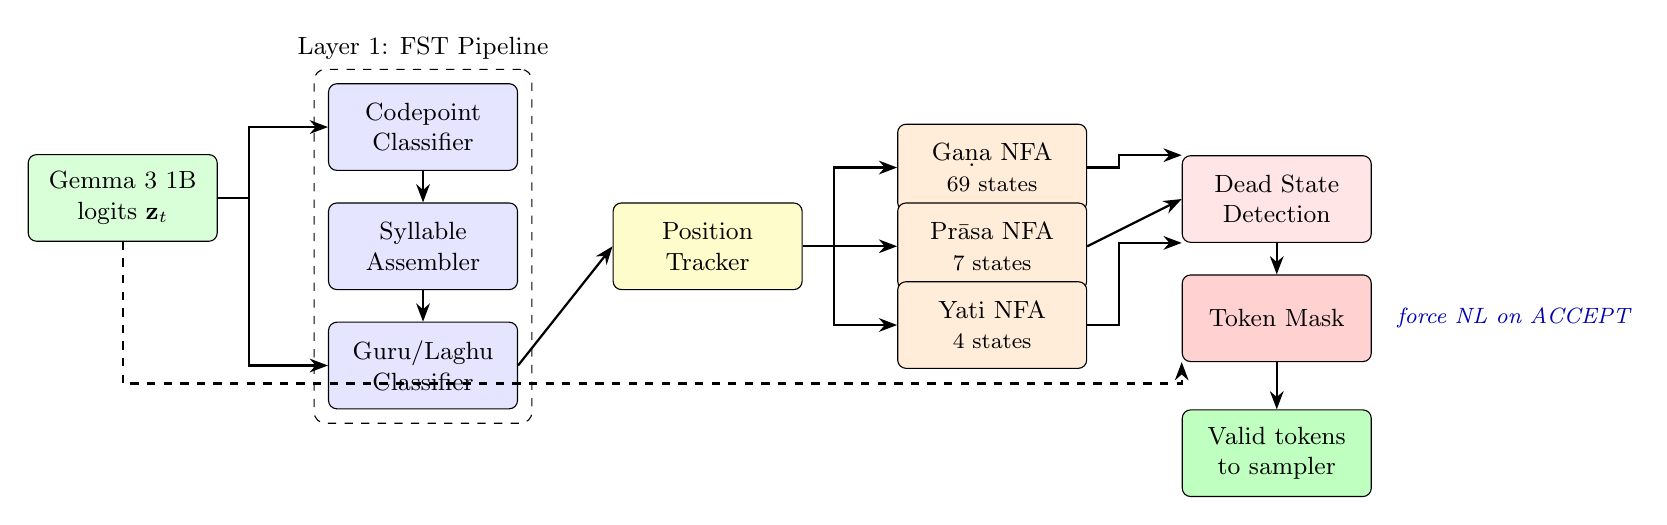
\begin{tikzpicture}[
  node distance=5mm and 10mm,
  box/.style={rectangle, draw, rounded corners=3pt, fill=blue!10,
              minimum width=24mm, minimum height=11mm,
              font=\small, align=center, inner sep=3pt},
  nfa/.style={rectangle, draw, rounded corners=3pt, fill=orange!15,
              minimum width=24mm, minimum height=11mm,
              font=\small, align=center, inner sep=3pt},
  >=Stealth
]
% LLM
\node[box, fill=green!15] (llm) {Gemma 3 1B\\logits $\mathbf{z}_t$};

% FST column
\node[box, right=14mm of llm, yshift=9mm]  (f1) {Codepoint\\Classifier};
\node[box, below=4mm of f1]                (f2) {Syllable\\Assembler};
\node[box, below=4mm of f2]                (f3) {Guru/Laghu\\Classifier};
\node[draw, dashed, rounded corners=4pt, fit=(f1)(f2)(f3),
      inner sep=5pt,
      label={[font=\small]above:{Layer 1: FST Pipeline}}] {};

% Position Tracker
\node[box, fill=yellow!20, right=12mm of f2] (pt) {Position\\Tracker};

% NFAs
\node[nfa, right=12mm of pt, yshift=10mm] (gn) {Ga\d{n}a NFA\\{\footnotesize 69 states}};
\node[nfa, right=12mm of pt]              (pn) {Pr\=asa NFA\\{\footnotesize 7 states}};
\node[nfa, right=12mm of pt, yshift=-10mm](yn) {Yati NFA\\{\footnotesize 4 states}};

% Dead State + Mask
\node[box, fill=red!10, right=12mm of pn, yshift=6mm]  (dead) {Dead State\\Detection};
\node[box, fill=red!18, below=4mm of dead]              (mask) {Token Mask};

% Valid output
\node[box, fill=green!25, below=6mm of mask] (out) {Valid tokens\\to sampler};

% Arrows: FST chain
\draw[->, thick] (f1) -- (f2);
\draw[->, thick] (f2) -- (f3);

% LLM -> FST
\draw[->, thick] (llm.east) -- ++(4mm,0) |- (f1.west);
\draw[->, thick] (llm.east) -- ++(4mm,0) |- (f3.west);

% FST -> Position Tracker
\draw[->, thick] (f3.east) -- (pt.west);

% Position Tracker -> NFAs
\draw[->, thick] (pt.east) -- ++(4mm,0) |- (gn.west);
\draw[->, thick] (pt.east) -- (pn.west);
\draw[->, thick] (pt.east) -- ++(4mm,0) |- (yn.west);

% NFAs -> Dead State
\draw[->, thick] (gn.east) -- ++(4mm,0) |- (dead.north west);
\draw[->, thick] (pn.east) -- (dead.west);
\draw[->, thick] (yn.east) -- ++(4mm,0) |- (dead.south west);

% Dead State -> Mask -> Output
\draw[->, thick] (dead) -- (mask);
\draw[->, thick] (mask) -- (out);

% Logits bypass (dashed)
\draw[->, dashed, thick] (llm.south) -- ++(0,-18mm) -| (mask.south west);

% Force NL annotation
\node[font=\footnotesize\itshape, text=blue!70!black,
      right=2mm of mask.east, anchor=west]
      {force NL on ACCEPT};

\end{tikzpicture}%
}
\caption{Symbolic Enforcer pipeline. Candidate tokens from Gemma~3~1B pass
through a two-stage FST pipeline (with inlined codepoint classifier), are
routed by the Position Tracker to three parallel NFAs (Ga\d{n}a, Pr\=asa,
Yati), and receive a boolean mask ($-\infty$ for invalid tokens) via dead
state detection. Dashed arrow: raw logits bypass path to the mask.}
\label{fig:enforcer}
\end{figure*}

% -------------------------------------------------------------------------
\section{Detailed Validation Results}
\label{app:validation}
% -------------------------------------------------------------------------

\subsection{Length Ratio Distribution}

Table~\ref{tab:lengthratio} reports the full distribution of length ratios
$r = |P|/|V|$ between Telugu prose meaning and poetic verse.

\begin{table}[H]
\centering
\small
\caption{Length ratio distribution ($n = 27{,}881$). Mean ratio: 1.63;
median: 1.61. Enforced bounds: $0.8 \leq r \leq 2.5$.}
\label{tab:lengthratio}
\begin{tabular}{lrr}
\toprule
\textbf{Ratio Range} & \textbf{Count} & \textbf{Share} \\
\midrule
0.50 -- 0.80 &      1 & $<$0.1\% \\
0.80 -- 1.00 &     78 &    0.3\% \\
1.00 -- 1.50 &  9,333 &   33.5\% \\
1.50 -- 2.00 & 15,449 &   55.4\% \\
2.00 -- 5.11 &  3,020 &   10.8\% \\
\midrule
\textbf{Pass rate} & \multicolumn{2}{r}{\textbf{99.1\% (27,633 / 27,881)}} \\
\bottomrule
\end{tabular}
\end{table}

\subsection{Extended Embedding Model Results}

Tables~\ref{tab:msbert} and~\ref{tab:l3cube} provide full per-pair results
for mSBERT-mpnet~\citep{reimers2020multilingual} and
L3Cube-IndicSBERT~\citep{deode2023l3cubeindicsbertsimpleapproachlearning} respectively.

\begin{table}[H]
\centering
\small
\caption{mSBERT-mpnet results across all text pairs ($n = 29{,}343$).}
\label{tab:msbert}
\begin{tabular}{lrrr}
\toprule
\textbf{Pair} & \textbf{Pass\%} & \textbf{Mean} & \textbf{Median} \\
\midrule
Poem -- Telugu meaning  & 63.7 & 0.685 & 0.701 \\
Poem -- English meaning &  4.4 & 0.424 & 0.422 \\
Telugu -- English       & 23.7 & 0.501 & 0.515 \\
\bottomrule
\end{tabular}
\end{table}

\begin{table}[H]
\centering
\small
\caption{L3Cube-IndicSBERT results across all text pairs ($n = 29{,}343$).}
\label{tab:l3cube}
\begin{tabular}{lrrr}
\toprule
\textbf{Pair} & \textbf{Pass\%} & \textbf{Mean} & \textbf{Median} \\
\midrule
Poem -- Telugu meaning  & 40.1 & 0.614 & 0.618 \\
Poem -- English meaning &  0.0 & 0.255 & 0.251 \\
Telugu -- English       & 21.0 & 0.579 & 0.585 \\
\bottomrule
\end{tabular}
\end{table}

\subsection{LaBSE Similarity Distribution}

Table~\ref{tab:labse_dist} gives the full distribution of LaBSE
Telugu-to-English cosine similarities.

\begin{table}[H]
\centering
\small
\caption{LaBSE Telugu meaning -- English meaning similarity
distribution ($n = 29{,}343$).}
\label{tab:labse_dist}
\begin{tabular}{lrr}
\toprule
\textbf{Range} & \textbf{Count} & \textbf{Share} \\
\midrule
0.00 -- 0.30 &      3 & $<$0.1\% \\
0.30 -- 0.50 &    592 &    2.0\% \\
0.50 -- 0.70 & 10,620 &   36.2\% \\
0.70 -- 0.85 & 16,294 &   55.5\% \\
0.85 -- 1.00 &  1,834 &    6.3\% \\
\bottomrule
\end{tabular}
\end{table}

\subsection{Lexical Diversity Metrics (Full)}

Table~\ref{tab:lexical-diversity} reports the complete corpus-level
and per-poem lexical-diversity metrics summarised inline in
Section~\ref{sec:validation}.

\begin{table}[H]
\centering
\small
\resizebox{\columnwidth}{!}{% % Forces the table to stay within column boundaries
\begin{tabular}{llrl}
\toprule
\textbf{Metric} & \textbf{Scope} & \textbf{Value} & \textbf{Reference} \\
\midrule
TTR ($V/N$)        & Corpus    & 0.491   & \citet{templin1957certain} \\
MATTR ($w{=}50$)   & Corpus    & 0.501   & \citet{covington2010} \\
Yule's $K$         & Corpus    & 3.497   & \citet{yule1944} \\
Honor\'{e}'s $H$   & Corpus    & 6164.7  & \citet{honore1979} \\
Hapax ratio ($V_1/V$) & Corpus & 0.804   & -- \\
Sichel's $S$ ($V_2/V$) & Corpus & 0.091 & \citet{sichel1975} \\
\midrule
Per-poem TTR (mean) & Poem     & 0.993   & -- \\
Per-poem MATTR ($w{=}2$, mean) & Poem & 1.000 & -- \\
Per-poem Yule's $K$ (mean) & Poem & 22.74 & -- \\
Per-poem Honor\'{e}'s $H$ (mean) & Poem & 2356.4 & -- \\
\midrule
Gemma~3 Telugu coverage & Subword & 74.4\% & -- \\
Per-poem subword TTR (mean)   & Subword & 0.897 & -- \\
\midrule
Exact duplicates   & Corpus    & 0       & -- \\
Near duplicates    & Corpus    & 160 (79 grp) & -- \\
\bottomrule
\end{tabular}%
}
\caption{Lexical diversity metrics for the validated Dvipada corpus (27,881 poems, 179,812 tokens, 88,295 types).}
\label{tab:lexical-diversity}
\end{table}

\subsection{LLM-as-a-Judge Per-Dimension Breakdown}

Table~\ref{tab:llmjudge} reports the per-dimension means and rating
distribution for the LLM-as-a-Judge evaluation summarised inline in
Section~\ref{sec:validation}.

\begin{table}[H]
\centering
\small
\caption{LLM-as-a-Judge evaluation ($n=250$). Columns give percentage of
samples at each rating. Mean total score: 24.25/25 (97.0\%).}
\label{tab:llmjudge}
\begin{tabular}{lrrrrr}
\toprule
\textbf{Dimension} & \textbf{Mean} & \textbf{5} & \textbf{4}
    & \textbf{3} & \textbf{$\leq$2} \\
\midrule
Semantic Fidelity  & 4.73 & 80.0 & 14.4 & 4.0 & 1.6 \\
Completeness       & 4.76 & 80.8 & 15.6 & 2.8 & 0.8 \\
Cultural Accuracy  & 4.89 & 93.6 &  2.8 & 2.4 & 1.2 \\
Telugu Linguistic  & 4.98 & 98.0 &  1.6 & 0.4 & 0.0 \\
English Linguistic & 4.90 & 90.4 &  8.8 & 0.8 & 0.0 \\
\bottomrule
\end{tabular}
\end{table}

\subsection{LLM-as-a-Judge Aggregate Score Distribution}

Table~\ref{tab:llmjudge_full} gives the full distribution of aggregate scores
(out of 25). Table~\ref{tab:llmjudge_sources} gives the stratified source
breakdown.

\begin{table}[H]
\centering
\small
\caption{LLM-as-a-Judge aggregate score distribution ($n = 250$).
Mean: 24.25/25 (97.0\%).}
\label{tab:llmjudge_full}
\begin{tabular}{rrr}
\toprule
\textbf{Score / 25} & \textbf{Count} & \textbf{Share} \\
\midrule
25 & 172 & 68.8\% \\
24 &  33 & 13.2\% \\
23 &  22 &  8.8\% \\
22 &   8 &  3.2\% \\
21 &   6 &  2.4\% \\
20 &   1 &  0.4\% \\
19 &   2 &  0.8\% \\
18 &   4 &  1.6\% \\
17 &   1 &  0.4\% \\
16 &   1 &  0.4\% \\
\bottomrule
\end{tabular}
\end{table}

\begin{table}[H]
\centering
\small
\caption{LLM-as-a-Judge stratified sample source distribution.}
\label{tab:llmjudge_sources}
\begin{tabular}{lr}
\toprule
\textbf{Source} & \textbf{Samples} \\
\midrule
Ranganatha Ramayanamu  & 42 \\
Basavapuranamu         & 42 \\
Dvipada Bhagavatamu 2  & 42 \\
Srirama Parinayamu     & 42 \\
Palanati Vira Charitra & 41 \\
Synthetic (LLM)        & 41 \\
\midrule
\textbf{Total}         & \textbf{250} \\
\bottomrule
\end{tabular}
\end{table}

% -------------------------------------------------------------------------
\section{Detailed End-to-End Benchmark Results}
\label{app:detailed_results}
% -------------------------------------------------------------------------

This appendix provides per-topic accuracy and per-poem efficiency
statistics for the twelve constrained-decoding configurations summarised
in Section~\ref{sec:results} (Tables~\ref{tab:dvipada-results}
and~\ref{tab:ragale-results}). All numbers are extracted directly from
the benchmark JSON files distributed with the project repository.

\subsection{Per-topic Dvipada accuracy}

Table~\ref{tab:dvipada-pertopic} reports the number of valid poems out of
34 seeds for each Telugu prompt. T1 = ``\textit{tallI prEma annintikaMTe
goppadi}'' (mother's love), T2 = ``\textit{hanumaMtuDu samudramunu dATi
laMkanu cErenu}'' (Hanuman crosses to Lanka), T3 =
``\textit{SrIrAmuDu sItAdEvini rakshiMcuTaku laMkaku veLLenu}'' (Rama
goes to Lanka). Each cell shows valid/34 ($p$\%).

\begin{table}[H]
\centering
\small
\caption{Per-topic poem accuracy on Dvipada (3 prompts $\times$ 34
seeds = 102 poems per row). The adapted Chandomitra port
\citep{jagadeeshan2026chandomitra} is included as an external baseline.}
\label{tab:dvipada-pertopic}
\resizebox{\columnwidth}{!}{%
\begin{tabular}{llrrr}
\toprule
\textbf{Model} & \textbf{Method} & \textbf{T1} & \textbf{T2} & \textbf{T3} \\
\midrule
\multicolumn{5}{l}{\textit{Adapted Chandomitra baseline}} \\
gemma3-1b-base   & chandomitra        &  0/34 (0.0)  &  0/34 (0.0)  &  1/34 (2.9)  \\
gemma3-1b-merged & chandomitra        &  2/34 (5.9)  &  4/34 (11.8) &  8/34 (23.5) \\
\midrule
\multicolumn{5}{l}{\textit{FST+NFA Symbolic Enforcer}} \\
gemma3-1b-base   & masking\_only      & 11/34 (32.4) & 14/34 (41.2) &  7/34 (20.6) \\
gemma3-1b-base   & masking\_backtrack & 32/34 (94.1) & 31/34 (91.2) & 30/34 (88.2) \\
gemma3-1b-base   & hybrid             & 34/34 (100.0)& 34/34 (100.0)& 34/34 (100.0)\\
\midrule
gemma3-1b-merged & masking\_only      & 12/34 (35.3) &  9/34 (26.5) & 16/34 (47.1) \\
gemma3-1b-merged & masking\_backtrack & 27/34 (79.4) & 28/34 (82.4) & 25/34 (73.5) \\
gemma3-1b-merged & hybrid             & 34/34 (100.0)& 34/34 (100.0)& 34/34 (100.0)\\
\bottomrule
\end{tabular}}
\end{table}

\subsection{Per-topic Ragale accuracy}

Table~\ref{tab:ragale-pertopic} reports the same breakdown for the three
Kannada topics.

\begin{table}[H]
\centering
\small
\caption{Per-topic poem accuracy on Ragale (3 prompts $\times$ 34
seeds = 102 poems per row).}
\label{tab:ragale-pertopic}
\resizebox{\columnwidth}{!}{%
\begin{tabular}{llrrr}
\toprule
\textbf{Model} & \textbf{Method} & \textbf{Bubbles} & \textbf{Moon} & \textbf{Rain} \\
\midrule
gemma3-1b-base & masking\_only      &  4/34 (11.8) &  4/34 (11.8) &  5/34 (14.7) \\
gemma3-1b-base & masking\_backtrack &  4/34 (11.8) &  4/34 (11.8) &  5/34 (14.7) \\
gemma3-1b-base & hybrid             & 17/34 (50.0) & 24/34 (70.6) & 28/34 (82.4) \\
\midrule
gemma3-1b-lora & masking\_only      & 33/34 (97.1) & 34/34 (100.0)& 31/34 (91.2) \\
gemma3-1b-lora & masking\_backtrack & 33/34 (97.1) & 34/34 (100.0)& 31/34 (91.2) \\
gemma3-1b-lora & hybrid             & 34/34 (100.0)& 34/34 (100.0)& 34/34 (100.0)\\
\bottomrule
\end{tabular}}
\end{table}

\subsection{Per-poem efficiency statistics}

Table~\ref{tab:efficiency-stats} reports the per-poem cost profile across
all twelve configurations: average tokens generated, average mask
computations, average backtracks, and total wall time over 102 poems.

\begin{table}[H]
\centering
\scriptsize
\caption{Per-poem efficiency profile across the twelve benchmark
configurations and the adapted Chandomitra baseline.
Tok = mean tokens generated; Mask = mean dynamic NFA mask
computations (n/a for the adapted Chandomitra port, which uses a
prefix-trie filter and does not maintain NFA state);
BT = mean backtrack count; Total = total wall time over 102 poems.}
\label{tab:efficiency-stats}
\resizebox{\columnwidth}{!}{%
\begin{tabular}{lllrrrr}
\toprule
\textbf{Lang} & \textbf{Model} & \textbf{Method} &
  \textbf{Tok} & \textbf{Mask} & \textbf{BT} & \textbf{Total (s)} \\
\midrule
Dvipada & gemma3-1b-base   & chandomitra        & 74.0 &  -- & 0.00 & 3865.5 \\
Dvipada & gemma3-1b-merged & chandomitra        & 97.3 &  -- & 0.00 & 6071.9 \\
\midrule
Dvipada & gemma3-1b-base   & masking\_only      & 52.1 & 50.2 & 0.00 &  355.7 \\
Dvipada & gemma3-1b-base   & masking\_backtrack & 34.0 & 49.1 & 7.10 &  352.1 \\
Dvipada & gemma3-1b-base   & hybrid             & 29.9 & 27.9 & 0.01 &  202.9 \\
Dvipada & gemma3-1b-merged & masking\_only      & 44.9 & 38.9 & 0.00 &  214.4 \\
Dvipada & gemma3-1b-merged & masking\_backtrack & 38.9 & 54.5 & 9.06 &  270.4 \\
Dvipada & gemma3-1b-merged & hybrid             & 34.0 & 28.0 & 0.00 &  156.0 \\
\midrule
Ragale  & gemma3-1b-base   & masking\_only      & 77.2 & 75.7 & 0.00 & 1092.9 \\
Ragale  & gemma3-1b-base   & masking\_backtrack & 77.2 & 75.7 & 0.00 &  386.0 \\
Ragale  & gemma3-1b-base   & hybrid             & 31.1 & 29.2 & 0.01 &  136.0 \\
Ragale  & gemma3-1b-lora   & masking\_only      & 25.8 & 23.8 & 0.00 &  145.2 \\
Ragale  & gemma3-1b-lora   & masking\_backtrack & 25.8 & 23.8 & 0.00 &  145.7 \\
Ragale  & gemma3-1b-lora   & hybrid             & 25.7 & 23.7 & 0.00 &  207.1 \\
\bottomrule
\end{tabular}}
\end{table}

\subsection{Methodology notes}

Each row in the tables above corresponds to a single benchmark script
invocation. Seeds follow the schedule $42 + 7k$ for $k\in[0,33]$ to
guarantee reproducibility while spanning the full RNG space the sampler
explores. The validator is the same chandas pipeline (FST + parallel
NFAs) used during corpus construction in Section~\ref{sec:validation},
so a poem labelled \textit{valid} here would also pass the inclusion
criterion that gated entry into the training corpus. Prompt templates
differ between the base and fine-tuned models (English instruction
template for LoRA models, Kannada/Telugu system-prompt template for base
models) so that each model is queried in the format closest to its
training distribution; both templates are described in
Section~\ref{sec:constrained}. The Ragale base model is the only
configuration where the same script run twice (masking\_only vs
masking\_backtrack) produces identical \emph{validity} numbers but
different \emph{wall times}, because backtracking can escape doomed
sequences earlier even when no alternative valid completion exists.

% -------------------------------------------------------------------------
\section{Kannada Script Conversion Details}
\label{app:kannada_details}
% -------------------------------------------------------------------------

\subsection{Character Coverage}

Table~\ref{tab:kannadamap} summarises the bidirectional converter's character
coverage by category, based on~\citet{nidamarthy2021comparative}.

\begin{table}[H]
\centering
\small
\caption{Kannada-Telugu bidirectional converter character
coverage~\citep{nidamarthy2021comparative}.}
\label{tab:kannadamap}
\begin{tabular}{lrr}
\toprule
\textbf{Category} & \textbf{Count} & \textbf{Resemblance} \\
\midrule
Consonants (high)    & 17 & 99\%          \\
Consonants (medium)  &  5 & 70--99\%      \\
Consonants (low)     &  5 & $<$70\%       \\
Remaining consonants &  8 & (varies)      \\
Vowels + signs       & 33 & 95--99\%      \\
Numerals             & 10 & 1:1 mapping   \\
\midrule
\textbf{Total}       & \textbf{78+} & \\
\bottomrule
\end{tabular}
\end{table}

\subsection{Output Schema}

Each entry in the converted Kannada dataset contains: the original Telugu
poem; the converted Kannada poem; Telugu and Kannada prose meanings; the
English meaning (unchanged); word-to-word glosses in Kannada script; a
conversion quality score; and per-entry counts of high-, medium-, and
low-resemblance characters used to compute the quality score.

\subsection{Limitations}

The conversion operates purely at the character level and cannot handle
script-specific ligature conventions or rendering differences between the two
scripts. Kannada-specific prosody rules are not yet validated; the converter
assumes that \textit{dvipada} metrical rules transfer identically from Telugu
to Kannada, which holds for shared Dravidian metres but would require
independent verification for Kannada-specific forms. Converted prose meanings
may sound unnatural when read as Kannada, though they function adequately as
conditioning prompts for generation.


Repo: \url{https://github.com/samvarankashyap/indicnuerosym}

% (Old algorithmic-syntax block removed)
\section{Constrained Decoding Algorithms}
\label{app:algorithms}

This appendix presents the formal pseudocode for the dead state
detection mechanism (Algorithm~\ref{alg:is-reachable}), the stateless
analysis subroutine (Algorithm~\ref{alg:analyze-text}), the dynamic
mask builder (Algorithm~\ref{alg:build-mask}), and the decoding
strategies referenced in Section~\ref{sec:constrained}: a stateless
\emph{Rejection Sampling} variant (Algorithm~\ref{alg:rejection-sampling},
reference only, not benchmarked), \emph{Masking with Backtracking}
(Algorithm~\ref{alg:masking-backtrack}), and \emph{Hybrid Mask +
Accept-State Re-ranking} (Algorithm~\ref{alg:hybrid}). The benchmarked
\emph{Masking-Only} strategy is Algorithm~\ref{alg:masking-backtrack}
run with the backtracking block disabled and is not shown separately.

\paragraph{Notation.}
$\theta$: language model;\;
$\mathcal{T}$: tokenizer;\;
$\mathbf{z}$: logit vector;\;
$\boldsymbol{\pi}$: probability distribution;\;
$\tau$: temperature;\;
$\mathbf{y}$: generated token sequence;\;
$\mathcal{S}$: \textsc{CompositeState} (incremental FST+NFA);\;
$\mathcal{B}$: active NFA branches;\;
$\mathcal{V}_{\text{tel}}$: pre-extracted Telugu token set;\;
$\mathbf{M}_s$: static mask ($0$ for Telugu/EOS, $-\infty$ elsewhere);\;
$\ell$: lines completed;\;
$\mathcal{C}$: checkpoint ring buffer;\;
$b, b_c$: total and consecutive backtrack counters.


% --------------------------------------------------------------------
% ALGORITHM 1: Dead State Detection
% --------------------------------------------------------------------

\begin{algorithm}[H]
\caption{\textsc{IsReachable}: Dead State Detection}
\label{alg:is-reachable}
\scriptsize
\begin{algorithmic}[1]
\Require $\mathcal{B}$: active NFA branches;\;
         $n$: syllables consumed in current line
\Ensure \textbf{true} iff any branch can reach \textsc{Accept}
        with $n_{\text{total}} \in [11, 15]$
\For{$(s, g, j, \mathcal{M}) \in \mathcal{B}$}
    \If{$s = \textsc{Accept}$}
        \State \textbf{if} $n \in \{11,\ldots,15\}$
               \textbf{then return true};\;
               \textbf{continue}
    \EndIf
    \State $r \gets |\textsc{Pool}(s)[g]| - j$
           \Comment{symbols left in current ga\d{n}a}
    \If{$s \le 2$} \Comment{Indra slot}
        \State $\ell_o \gets r + (2{-}s) \cdot 3 + 2$
               \Comment{min to accept}
        \State $h \gets r + (2{-}s) \cdot 4 + 3$
               \Comment{max to accept}
    \Else \Comment{Surya slot ($s = 3$)}
        \State $\ell_o \gets r$;\; $h \gets r$
    \EndIf
    \If{$n + \ell_o \le 15$ \textbf{and} $n + h \ge 11$}
        \State \Return \textbf{true}
    \EndIf
\EndFor
\State \Return \textbf{false} \Comment{all branches doomed}
\end{algorithmic}
\end{algorithm}


% --------------------------------------------------------------------
% ALGORITHM 2: AnalyzeText
% --------------------------------------------------------------------

\begin{algorithm}[H]
\caption{\textsc{AnalyzeText}: Stateless FST+NFA Analysis}
\label{alg:analyze-text}
\scriptsize
\begin{algorithmic}[1]
\Require Unicode string $w$ (prefix-stripped)
\Ensure $(\text{alive},\; \ell_c,\; \text{acc},\; n,\; \mathcal{B})$
\State Init fresh \textsc{SyllAssembler} $A$,
       \textsc{GuruLaghuClassifier} $G$
\State $\mathcal{B} \gets \textsc{SpawnSlot}(0, ())$;\;
       $\ell_c \gets 0$;\; $\text{mk} \gets [\,]$
\For{item $\in A.\text{process}(w)$}
    \If{item $= \text{``\textbackslash n''}$}
        \State Flush $G$; advance $\mathcal{B}$ with labels
        \If{$\exists\, (\textsc{Accept},*,*,*) \in \mathcal{B}$}
            \State $\ell_c \mathrel{+}= 1$
        \EndIf
        \State $\mathcal{B} \gets \textsc{SpawnSlot}(0,())$;\;
               $\text{mk} \gets [\,]$
    \ElsIf{item $= \text{``\textvisiblespace''}$}
        \State Flush boundary; advance $\mathcal{B}$
    \Else
        \State Feed syllable to $G$; advance $\mathcal{B}$
    \EndIf
\EndFor
\State Flush remaining; advance $\mathcal{B}$
\State $n \gets |\text{mk}|$
\State $\text{acc} \gets \exists\,(\textsc{Accept},*,*,*)
       \in \mathcal{B} \,\wedge\, n \in \{11{\ldots}15\}$
\State $\text{alive} \gets \textsc{IsReachable}(\mathcal{B}, n)
       \vee (\ell_c \ge 2)$
\State \Return $(\text{alive},\; \ell_c,\; \text{acc},\; n,\; \mathcal{B})$
\end{algorithmic}
\end{algorithm}


% --------------------------------------------------------------------
% ALGORITHM 3: BuildGanaMask
% --------------------------------------------------------------------

\begin{algorithm}[H]
\caption{\textsc{BuildGanaMask}: Dynamic NFA Token Mask}
\label{alg:build-mask}
\scriptsize
\begin{algorithmic}[1]
\Require $\sigma$: \textsc{CompositeState} snapshot;\;
         $\mathcal{V}_{\text{tel}} = (\text{ids}, \text{texts})$
\Ensure $\mathcal{V}_v$: token IDs keeping all NFAs alive
\State $\mathcal{V}_v \gets \emptyset$
\For{$(\text{tid}, \text{txt}) \in
     \text{zip}(\text{ids}, \text{texts})$}
    \State $\mathcal{S}' \gets
           \textsc{FromSnapshot}(\sigma)$
    \State $\mathcal{S}'.\text{feed\_token}(\text{txt})$;\;
           $\mathcal{S}'.\text{flush}()$
    \If{$\mathcal{S}'.\text{is\_alive}()$}
        \Comment{ga\d{n}a $\wedge$ pr\=asa $\wedge$ yati}
        \State $\mathcal{V}_v \gets \mathcal{V}_v
               \cup \{\text{tid}\}$
    \EndIf
\EndFor
\State \Return $\mathcal{V}_v$
\end{algorithmic}
\end{algorithm}


% --------------------------------------------------------------------
% ALGORITHM 4: Rejection Sampling
% --------------------------------------------------------------------

\begin{algorithm}[H]
\caption{Strategy~1: Rejection Sampling}
\label{alg:rejection-sampling}
\scriptsize
\begin{algorithmic}[1]
\Require $\theta$, $\mathcal{T}$, $\tau$, $K$, $p$
\Ensure Two-line Dvipada poem text
\State $\mathbf{y} \gets [\,]$;\; $\ell \gets 0$
\While{$\ell < 2$}
    \State $\boldsymbol{\pi} \gets
           \text{softmax}(\theta(\mathbf{y})/\tau)$;\;
           sort desc
    \State $\text{st} \gets \textsc{AnalyzeText}(
           \textsc{StripPrefix}(
           \mathcal{T}.\text{dec}(\mathbf{y})))$
    \State $\ell \gets \text{st}.\ell_c$;\;
           \textbf{if} $\ell \ge 2$ \textbf{then break}
    \State \Comment{\textit{Force newline on completion/overshoot}}
    \If{$\text{st.acc} \wedge \text{st}.n \in \{11{\ldots}15\}$}
        \State $\mathbf{y} \gets \mathbf{y} \,\|\,
               [\textsc{NL}]$;\; \textbf{continue}
    \EndIf
    \If{$\text{st}.n > 15 \wedge \neg\text{st.acc}$}
        \State $\mathbf{y} \gets \mathbf{y} \,\|\,
               [\textsc{NL}]$;\; \textbf{continue}
    \EndIf
    \State $K' \gets K$;\;
           \textbf{if} $\text{st}.n \ge 8$
           \textbf{then} $K' \gets 2K$
    \State \Comment{\textit{Rejection loop over top-$K'$}}
    \State $\mathcal{V}_{\text{acc}} \gets \emptyset$;\;
           $\mathcal{V}_{\text{alv}} \gets \emptyset$
    \For{$k = 1$ \textbf{to} $K'$}
        \State $c \gets \pi_k$;\;
               \textbf{if} $\boldsymbol{\pi}(c) < 10^{-8}$
               \textbf{then break}
        \State \textbf{if} $c = \textsc{Eos} \wedge
               \ell \ge 2$ \textbf{then} select $c$;
               \textbf{break}
        \State \textbf{if} $\neg\textsc{IsTelugu}(
               \mathcal{T}.\text{dec}(c))$
               \textbf{then continue}
        \State $r \gets \textsc{AnalyzeText}(
               \textsc{StripPrefix}(
               \mathcal{T}.\text{dec}(
               \mathbf{y} \,\|\, [c])))$
               \Comment{full re-analysis}
        \State \textbf{if} $\neg r.\text{alive}$
               \textbf{then continue}
        \State \textbf{if} ``\textbackslash n''
               $\in \mathcal{T}.\text{dec}(c)
               \wedge r.\ell_c \le \ell$
               \textbf{then continue}
        \State \textbf{if} $r.n > 15 \wedge
               \neg r.\text{acc}$
               \textbf{then continue}
        \If{$r.\text{acc} \wedge r.n
            \in \{11{\ldots}15\}$}
            \State $\mathcal{V}_{\text{acc}} \gets
                   \mathcal{V}_{\text{acc}} \cup
                   \{(c, \boldsymbol{\pi}(c))\}$
        \EndIf
        \State $\mathcal{V}_{\text{alv}} \gets
               \mathcal{V}_{\text{alv}} \cup
               \{(c, \boldsymbol{\pi}(c))\}$
        \State \textbf{if} $|\mathcal{V}_{\text{acc}}|
               \ge 5$ \textbf{then break}
    \EndFor
    \State \Comment{\textit{Select from best candidate set}}
    \State $\mathcal{V} \gets
           \mathcal{V}_{\text{acc}}$ if $\neq\emptyset$,
           else $\mathcal{V}_{\text{alv}}$
    \If{$\mathcal{V} \ne \emptyset$}
        \State Top-$p$ filter;\;
               $\text{chosen} \gets$ weighted sample
               from $\mathcal{V}$
    \Else
        \State \Comment{Exhaustive fallback (500 tokens)}
        \For{$k = 1$ \textbf{to} $500$}
            \If{$\textsc{IsTelugu}(\mathcal{T}.\text{dec}(\pi_k))$}
                \State $r \gets \textsc{AnalyzeText}(
                       \textsc{StripPrefix}(
                       \mathcal{T}.\text{dec}(
                       \mathbf{y} \,\|\, [\pi_k])))$
                \If{$r.\text{alive} \wedge
                    (r.n \le 15 \vee r.\text{acc})$}
                    \State $\text{chosen} \gets \pi_k$;\;
                           \textbf{break}
                \EndIf
            \EndIf
        \EndFor
    \EndIf
    \State $\mathbf{y} \gets \mathbf{y} \,\|\,
           [\text{chosen}]$
\EndWhile
\State \Return $\mathcal{T}.\text{dec}(\mathbf{y})$
\end{algorithmic}
\end{algorithm}


% --------------------------------------------------------------------
% ALGORITHM 5: Logit Masking with Backtracking
% --------------------------------------------------------------------

\begin{algorithm}[H]
\caption{Strategy~2: Logit Masking with Backtracking}
\label{alg:masking-backtrack}
\scriptsize
\begin{algorithmic}[1]
\Require $\theta$, $\mathcal{T}$, $\mathcal{V}_{\text{tel}}$,
         $\mathbf{M}_s$, $\tau$,
         $\tau_{\max}{=}1.2$,
         $\Delta\tau{=}0.15$, $D{=}6$
\Ensure Two-line Dvipada poem text
\State $\mathbf{y} \gets [\,]$;\;
       $\mathcal{S} \gets$ new \textsc{CompositeState}();\;
       $\ell \gets 0$;\; $\tau_c \gets \tau$
\State $\mathcal{C} \gets [\,]$;\;
       $b \gets 0$;\; $b_c \gets 0$;\; $d \gets 0$
       \Comment{ring buffer, counters}
\For{$t = 1$ \textbf{to} $T_{\max}$}
    \If{$\ell \ge 2$} \textbf{break} \EndIf
    \State $\mathbf{z} \gets \theta(\mathbf{y})/\tau_c
           + \mathbf{M}_s$
           \Comment{static mask}
    \State \Comment{\textit{Checkpoint every 3 tokens}}
    \If{$t \bmod 3 = 0$}
        \State $\mathcal{C}.\text{push}(t,\;
               \mathcal{S}.\text{snap}(),\;
               |\mathbf{y}|,\; \ell,\; \tau_c)$
        \State \textbf{if} $|\mathcal{C}| > 15$
               \textbf{then}
               $\mathcal{C} \gets \mathcal{C}[-15:]$
    \EndIf
    \State \Comment{\textit{Force newline on ACCEPT}}
    \State $\mathcal{S}_f \gets \text{clone}(\mathcal{S})$;\;
           $\mathcal{S}_f.\text{flush}()$
    \If{$\mathcal{S}_f.\text{has\_accept}()$}
        \State $\mathcal{S}.\text{feed}(
               \text{``\textbackslash n''})$;\;
               $\ell \gets \mathcal{S}.\ell_c$;\;
               $\mathbf{y} \gets \mathbf{y} \,\|\,
               [\textsc{NL}]$
        \State $b_c \gets 0$;\; \textbf{continue}
    \EndIf
    \State \Comment{\textit{Build dynamic NFA mask}}
    \State $\sigma \gets \mathcal{S}.\text{snap}()$;\;
           $\mathcal{V}_v \gets
           \textsc{BuildGanaMask}(\sigma,
           \mathcal{V}_{\text{tel}})$
    \State \Comment{\textit{Filter spurious newlines}}
    \If{$\textsc{NL} \in \mathcal{V}_v$}
        \State $\mathcal{S}' \gets
               \textsc{FromSnap}(\sigma)$;\;
               $\mathcal{S}'.\text{feed}(
               \text{``\textbackslash n''})$
        \If{$\mathcal{S}'.\ell_c \le \ell$}
            \State $\mathcal{V}_v \gets
                   \mathcal{V}_v \setminus
                   \{\textsc{NL}\}$
        \EndIf
    \EndIf
    \State \Comment{\textit{Backtrack if dead end}}
    \If{$(|\mathcal{V}_v| < 3 \;\vee\;
         \mathcal{S}_f.n > 15)$
         \textbf{and} $|\mathcal{C}| > 0$
         \textbf{and} $b < 30$}
        \State $b \mathrel{+}= 1$;\;
               $b_c \mathrel{+}= 1$
        \State Pop $\min(b_c, |\mathcal{C}|)$
               from $\mathcal{C}$
        \State Restore $\mathcal{S}, \mathbf{y},
               \ell, t$ from last popped
        \State $\tau_c \gets \min(\text{ckpt}.\tau
               + \Delta\tau \cdot b_c,\;
               \tau_{\max})$
               \Comment{escalate}
        \State $d \gets D$;\;
               $\textsc{Seed}(\text{seed}
               + b \cdot 1337)$;\;
               \textbf{continue}
    \EndIf
    \State \Comment{\textit{Apply dynamic mask and sample}}
    \State $\mathbf{M}_d[i] \gets 0$ if
           $i \in \mathcal{V}_v$, else $-\infty$
    \State $\mathbf{z} \gets \mathbf{z} + \mathbf{M}_d$;\;
           $\boldsymbol{\pi} \gets
           \text{softmax}(\mathbf{z})$
    \State $\text{chosen} \gets
           \text{sample}(\boldsymbol{\pi}, p)$
    \State \Comment{\textit{Commit token}}
    \State $\mathbf{y} \gets \mathbf{y} \,\|\,
           [\text{chosen}]$;\;
           $\mathcal{S}.\text{feed\_token}(
           \mathcal{T}.\text{dec}(\text{chosen}))$
    \State $\ell \gets \mathcal{S}.\ell_c$;\;
           $b_c \gets 0$
    \State \Comment{\textit{Temperature decay}}
    \If{$d > 0$}
        \State $d \mathrel{-}= 1$;\;
               \textbf{if} $d = 0$
               \textbf{then} $\tau_c \gets \tau$
    \EndIf
\EndFor
\State \Return $\mathcal{T}.\text{dec}(\mathbf{y})$
\end{algorithmic}
\end{algorithm}


% --------------------------------------------------------------------
% ALGORITHM 6: Hybrid (Mask + Accept-State Re-ranking)
% --------------------------------------------------------------------

\begin{algorithm}[H]
\caption{Strategy~3: Hybrid (Mask + Accept-State Re-ranking)}
\label{alg:hybrid}
\scriptsize
\begin{algorithmic}[1]
\Require $\theta$, $\mathcal{T}$, $\mathcal{V}_{\text{tel}}$,
         $\mathbf{M}_s$, $\tau$, $K_r{=}100$
\Ensure Two-line Dvipada poem text
\State $\mathbf{y} \gets [\,]$;\;
       $\mathcal{S} \gets$ new \textsc{CompositeState}();\;
       $\ell \gets 0$;\; $\tau_c \gets \tau$
\State $\mathcal{C} \gets [\,]$;\;
       $b \gets 0$;\; $b_c \gets 0$
\For{$t = 1$ \textbf{to} $T_{\max}$}
    \If{$\ell \ge 2$} \textbf{break} \EndIf
    \State $\mathbf{z} \gets \theta(\mathbf{y})/\tau_c
           + \mathbf{M}_s$
    \State \textbf{if} $t \bmod 3 = 0$
           \textbf{then} checkpoint
           $\mathcal{C}$ (cap 15)
    \State \Comment{\textit{Force newline on ACCEPT}}
    \State $\mathcal{S}_f \gets \text{clone}(\mathcal{S})$;\;
           $\mathcal{S}_f.\text{flush}()$
    \If{$\mathcal{S}_f.\text{has\_accept}()$}
        \State $\mathcal{S}.\text{feed}(
               \text{``\textbackslash n''})$;\;
               $\ell \gets \mathcal{S}.\ell_c$;\;
               $\mathbf{y} \gets \mathbf{y} \,\|\,
               [\textsc{NL}]$;\;
               $b_c \gets 0$;\;
               \textbf{continue}
    \EndIf
    \State \Comment{\textit{Build + apply dynamic NFA mask}}
    \State $\sigma \gets \mathcal{S}.\text{snap}()$;\;
           $\mathcal{V}_v \gets
           \textsc{BuildGanaMask}(\sigma,
           \mathcal{V}_{\text{tel}})$
    \State Filter spurious newlines
           (as Alg.~\ref{alg:masking-backtrack})
    \State $\mathbf{M}_d[i] \gets 0$ if
           $i \in \mathcal{V}_v$, else $-\infty$;\;
           $\mathbf{z} \gets \mathbf{z} + \mathbf{M}_d$
    \State $\boldsymbol{\pi} \gets
           \text{softmax}(\mathbf{z})$;\;
           sort desc
    \State \Comment{\textit{Accept-state re-ranking pass over top-$K_r$
           from masked dist.}}
    \State $\mathcal{V}_{\text{acc}} \gets \emptyset$;\;
           $\mathcal{V}_{\text{alv}} \gets \emptyset$
    \For{$k = 1$ \textbf{to} $K_r$}
        \State $c \gets \pi_k$;\;
               \textbf{if} $\boldsymbol{\pi}(c) < 10^{-8}$
               \textbf{then break}
        \State \textbf{if} $c = \textsc{Eos} \wedge
               \ell \ge 2$ \textbf{then} select $c$;
               \textbf{break}
        \State \Comment{Clone state, simulate candidate}
        \State $\mathcal{S}' \gets
               \textsc{FromSnap}(\sigma)$
        \State \textbf{for each} ch $\in
               \mathcal{T}.\text{dec}(c)$
               \textbf{do} $\mathcal{S}'.\text{feed}(
               \text{ch})$
        \State $\mathcal{S}'_f \gets
               \text{clone}(\mathcal{S}')$;\;
               $\mathcal{S}'_f.\text{flush}()$
        \State \textbf{if} $\neg\mathcal{S}'_f
               .\text{alive}()$
               \textbf{then continue}
        \State \textbf{if} ``\textbackslash n''
               $\in \mathcal{T}.\text{dec}(c) \wedge
               \mathcal{S}'.\ell_c \le \ell$
               \textbf{then continue}
        \State \textbf{if} $\mathcal{S}'_f.n > 15
               \wedge \neg\mathcal{S}'_f.\text{acc}()$
               \textbf{then continue}
        \If{$\mathcal{S}'_f.\text{has\_accept}()$}
            \State $\mathcal{V}_{\text{acc}} \gets
                   \mathcal{V}_{\text{acc}} \cup
                   \{(c, \boldsymbol{\pi}(c))\}$
        \EndIf
        \State $\mathcal{V}_{\text{alv}} \gets
               \mathcal{V}_{\text{alv}} \cup
               \{(c, \boldsymbol{\pi}(c))\}$
        \State \textbf{if} $|\mathcal{V}_{\text{acc}}|
               \ge 3$ \textbf{then break}
        \State \textbf{if} $|\mathcal{V}_{\text{alv}}|
               \ge 10 \wedge
               \mathcal{V}_{\text{acc}} = \emptyset$
               \textbf{then break}
    \EndFor
    \State \Comment{\textit{Select or backtrack}}
    \State $\mathcal{V} \gets
           \mathcal{V}_{\text{acc}}$ if $\neq\emptyset$,
           else $\mathcal{V}_{\text{alv}}$
    \If{$\mathcal{V} \ne \emptyset$}
        \State Normalize;\;
               $\text{chosen} \gets$ weighted sample
    \ElsIf{$|\mathcal{C}| > 0 \wedge b < 30$}
        \State $b \mathrel{+}= 1$;\;
               $b_c \mathrel{+}= 1$;\;
               pop $\min(b_c, |\mathcal{C}|)$
               from $\mathcal{C}$
        \State Restore $\mathcal{S}, \mathbf{y},
               \ell, t$;\;
               $\tau_c \gets \min(\text{ckpt}.\tau
               {+} \Delta\tau {\cdot} b_c,\,
               \tau_{\max})$
        \State $\textsc{Seed}(\text{seed}
               {+} b {\cdot} 1337)$;\;
               \textbf{continue}
    \Else
        \State $\text{chosen} \gets \pi_1$
               \Comment{last resort}
    \EndIf
    \State $\mathbf{y} \gets \mathbf{y} \,\|\,
           [\text{chosen}]$;\;
           $\mathcal{S}.\text{feed\_token}(
           \mathcal{T}.\text{dec}(\text{chosen}))$;\;
           $\ell \gets \mathcal{S}.\ell_c$;\;
           $b_c \gets 0$
\EndFor
\State \Return $\mathcal{T}.\text{dec}(\mathbf{y})$
\end{algorithmic}
\end{algorithm}


% --------------------------------------------------------------------
% FIGURE 2: Decoding Strategies overview (relocated from §8)
% --------------------------------------------------------------------

\begin{figure*}[h]
\centering
\resizebox{\textwidth}{!}{%
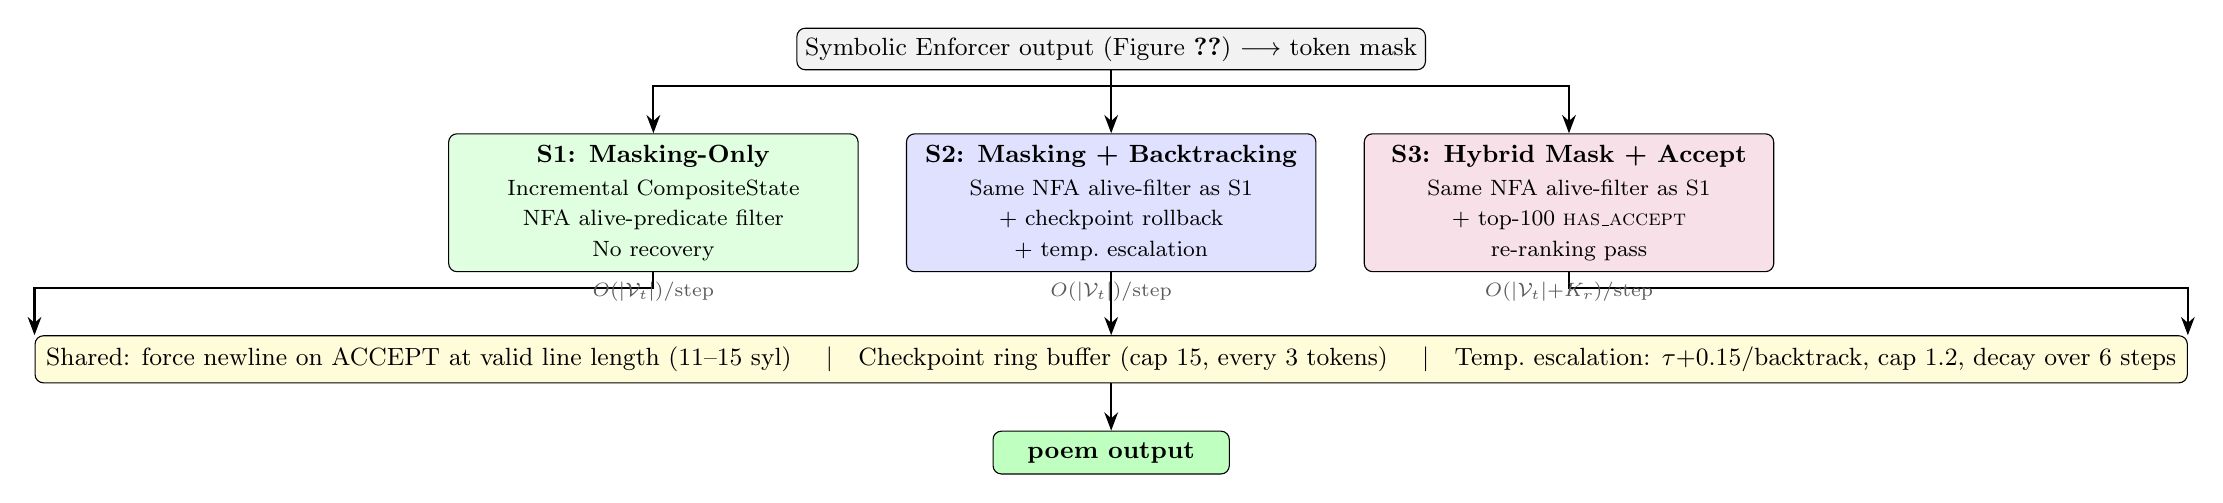
\begin{tikzpicture}[
  node distance=5mm and 8mm,
  sbox/.style={rectangle, draw, rounded corners=3pt,
               minimum width=52mm, minimum height=16mm,
               font=\small, align=center, inner sep=4pt},
  >=Stealth
]
% Three strategy boxes side by side
\node[sbox, fill=green!12]
    (s1) {\textbf{S1: Masking-Only}\\[1pt]
          \footnotesize Incremental CompositeState\\
          \footnotesize NFA alive-predicate filter\\
          \footnotesize No recovery};

\node[sbox, fill=blue!12, right=6mm of s1]
    (s2) {\textbf{S2: Masking + Backtracking}\\[1pt]
          \footnotesize Same NFA alive-filter as S1\\
          \footnotesize + checkpoint rollback\\
          \footnotesize + temp.\ escalation};

\node[sbox, fill=purple!12, right=6mm of s2]
    (s3) {\textbf{S3: Hybrid Mask + Accept}\\[1pt]
          \footnotesize Same NFA alive-filter as S1\\
          \footnotesize + top-100 \textsc{has\_accept}\\
          \footnotesize re-ranking pass};

% Shared box below
\node[rectangle, draw, rounded corners=3pt, fill=yellow!15,
      font=\small, align=center, inner sep=4pt,
      minimum width=80mm, below=8mm of s2]
    (shared) {Shared: force newline on ACCEPT at valid line length
              (11--15 syl) \quad\textbar\quad
              Checkpoint ring buffer (cap 15, every 3 tokens) \quad\textbar\quad
              Temp.\ escalation: $\tau {+} 0.15$/backtrack, cap $1.2$, decay over 6 steps};

% Enforcer input label above
\node[rectangle, draw, rounded corners=3pt, fill=gray!10,
      font=\small, align=center, inner sep=3pt,
      minimum width=50mm, above=8mm of s2]
    (input) {Symbolic Enforcer output (Figure~\ref{fig:enforcer})
             $\longrightarrow$ token mask};

% Arrows from enforcer to strategies
\draw[->, thick] (input.south) -- ++(0,-2mm) -| (s1.north);
\draw[->, thick] (input.south) -- (s2.north);
\draw[->, thick] (input.south) -- ++(0,-2mm) -| (s3.north);

% Strategies to shared
\draw[->, thick] (s1.south) -- ++(0,-2mm) -| (shared.north west);
\draw[->, thick] (s2.south) -- (shared.north);
\draw[->, thick] (s3.south) -- ++(0,-2mm) -| (shared.north east);

% Output
\node[rectangle, draw, rounded corners=3pt, fill=green!25,
      font=\small\bfseries, align=center, inner sep=4pt,
      minimum width=30mm, below=6mm of shared]
    (out) { poem output};
\draw[->, thick] (shared.south) -- (out.north);

% Cost labels
\node[font=\scriptsize, text=gray!70!black, below=0mm of s1.south,
      anchor=north] {$O(|\mathcal{V}_t|)$/step};
\node[font=\scriptsize, text=gray!70!black, below=0mm of s2.south,
      anchor=north] {$O(|\mathcal{V}_t|)$/step};
\node[font=\scriptsize, text=gray!70!black, below=0mm of s3.south,
      anchor=north] {$O(|\mathcal{V}_t|{+}K_r)$/step};

\end{tikzpicture}%
}% end resizebox
\caption{Three constrained decoding strategies using the Symbolic
Enforcer. All three share the same per-step NFA
alive-predicate filter via \textsc{BuildGanaMask} over the
$\sim$1{,}822 Telugu tokens ($O(|\mathcal{V}_{\text{tel}}|)$ per step,
sequence-length independent). (S1)~Masking-only: no recovery, no
re-ranking. (S2)~Masking with backtracking: adds checkpoint rollback
and temperature escalation when the alive set collapses. (S3)~Hybrid:
adds a second NFA pass over the top-$K_r{=}100$ masked candidates
that re-ranks by \textsc{has\_accept} (line-completion) preference;
backtracking is retained only as a rare fallback.}
\label{fig:strategies}
\end{figure*}


% --------------------------------------------------------------------
% COMPARISON TABLE
% --------------------------------------------------------------------

\begin{table}[H]
\centering
\scriptsize
\caption{Comparison of constrained decoding strategies. The
first column (Stateless Rejection) is the reference variant of
Algorithm~\ref{alg:rejection-sampling} (not benchmarked in
Section~\ref{sec:results}); the last two columns correspond to the
benchmarked Masking+Backtracking and Hybrid strategies. All three
share the same NFA machinery but differ in how the NFAs are consulted
per step.}
\label{tab:strategy-comparison}
\begin{tabular}{lccc}
\toprule
\textbf{Property}
    & \textbf{Stateless Rej.}
    & \textbf{Mask.\,+\,BT}
    & \textbf{Hybrid} \\
    & (Alg~\ref{alg:rejection-sampling})
    & (Alg~\ref{alg:masking-backtrack})
    & (Alg~\ref{alg:hybrid}) \\
\midrule
State track.
    & Stateless
    & Incremental
    & Incremental \\
Per-step
    & $O(KL)$
    & $O(|\mathcal{V}_t|)$
    & $O(|\mathcal{V}_t|{+}K_r)$ \\
Seq.\ dep.
    & Yes
    & No
    & No \\
Reject.\ set
    & Top-$K$
    & All Telugu
    & All Telugu \\
Recovery
    & Exhaust.
    & Backtrack
    & Backtrack \\
Temp.\ adapt.
    & None
    & Escalation
    & Escalation \\
Constraints
    & Ga\d{n}a reach.
    & All 3 (alive)
    & All 3 (alive) \\
Accept re-rank
    & $\checkmark$ (first hit)
    & $\times$
    & $\checkmark$ (top-$100$) \\
\bottomrule
\end{tabular}
\end{table}


% -------------------------------------------------------------------------
\section{Ragale Constrained Decoding: Construction Details}
\label{app:ragale_construction}
% -------------------------------------------------------------------------

This appendix provides full construction details for the Kannada
\textit{utsaha ragale} variant of the Symbolic Enforcer summarised in
Section~\ref{sec:ragale_decoding}. The FST pipeline (Syllable Assembler
and Guru/Laghu Classifier) is architecturally identical to the Dvipada
pipeline; only the Unicode codepoint sets change from Telugu
(U+0C00--U+0C7F) to Kannada (U+0C80--U+0CFF). The five
guru/laghu classification rules (Section~\ref{sec:fst}) apply unchanged.

\subsection{Structural Differences from Dvipada}

Table~\ref{tab:dvipada_vs_ragale} summarises the key differences
between the two metres' constraint specifications.

\begin{table}[h]
\centering
\small
\caption{Dvipada vs.\ Ragale constraint comparison.}
\label{tab:dvipada_vs_ragale}
\resizebox{\columnwidth}{!}{%
\begin{tabular}{lll}
\toprule
\textbf{Aspect} & \textbf{Dvipada (Telugu)} & \textbf{Ragale (Kannada)} \\
\midrule
Ga\d{n}a patterns  & 8 (6 Indra + 2 Surya) & 2 (III, IIU) \\
Formal language     & $(6\text{ pat.})^3 \cdot (2\text{ pat.})$ & $(\text{III}\mid\text{IIU})^3 \cdot \text{IIU}$ \\
Syllables/line      & 11--15 (variable)     & 12 (fixed) \\
Ga\d{n}a sizes      & 2--4 syllables        & 3 (uniform) \\
Pr\=asa             & 7 states, 3 equiv.\ groups & 7 states, 2 equiv.\ groups \\
Yati                & 4 states (optional)   & Not used \\
Guru ending         & Implicit              & Enforced (ga\d{n}a 4 = IIU) \\
\bottomrule
\end{tabular}%
}
\end{table}

\subsection{Ga\d{n}a NFA for Ragale}

The Ragale Ga\d{n}a NFA validates each line against the regular pattern:
\begin{equation}
L_{\text{line}} = (\text{III} \mid \text{IIU})^3 \cdot \text{IIU}
\end{equation}

Only two ga\d{n}a patterns are permitted (Table~\ref{tab:utsaha_ganas}):
III (three \textit{laghu}) at positions 1--3, and IIU (two \textit{laghu}
+ one \textit{guru}) at all four positions. Position~4 is constrained to
IIU, structurally enforcing the \textit{guru} ending rule. This yields
exactly $2^3 = 8$ valid line patterns, all of length 12 syllables.

The NFA has \textbf{22 states}: slots 0--2 each spawn 2 candidate \textit{ga\d{n}as}
with 3 sub-positions ($2 \times 3 \times 3 = 18$), slot~3 spawns only
IIU ($1 \times 3 = 3$), plus 1 \textsc{accept} state. Compared to the
Dvipada Ga\d{n}a NFA (69 states), the Ragale variant achieves a
$3.1\times$ reduction.

Dead state detection (Algorithm~\ref{alg:is-reachable}) simplifies because
all \textit{ga\d{n}as} are exactly 3 syllables: $\textit{min\_dist}(s) =
\textit{max\_dist}(s) = (3 - j) + (3 - s) \times 3$, where $j$ is the
sub-position and $s$ is the slot index.

\subsection{Pr\=asa and Guru Ending}

The Pr\=asa NFA retains the same 7-state structure
(\textsc{line1\_syl0} through \textsc{accept}/\textsc{reject}) with two
Kannada-specific equivalence groups: laterals
$\{$\d{l}a~$\leftrightarrow$~la$\}$ and sibilants
$\{$\'{s}a~$\leftrightarrow$~\d{s}a~$\leftrightarrow$~sa$\}$.
The rhotic group ($\{$\d{r}a, ra$\}$) present in Telugu is absent in
Kannada, reducing from 3 to 2 equivalence pairs.

The \textit{guru} ending constraint is not checked as a separate rule;
it is structurally guaranteed by the Ga\d{n}a NFA's restriction of
position~4 to IIU, whose final syllable is always \textit{guru} (U).

\subsection{State Budget}

Table~\ref{tab:ragale_states} shows the Ragale state budget.

\begin{table}[h]
\centering
\small
\caption{State budget for the Ragale constrained decoding system.}
\label{tab:ragale_states}
\begin{tabular}{llr}
\toprule
\textbf{Component} & \textbf{Type} & \textbf{States} \\
\midrule
Codepoint Classifier  & Stateless & 0 (inlined) \\
Syllable Assembler    & Mealy FST & 4 \\
Guru/Laghu Classifier & Mealy FST & 2 \\
Position Tracker      & Controller & 3 (counter) \\
Ga\d{n}a NFA          & NFA & 22 \\
Pr\=asa NFA           & NFA & 7 \\
Yati NFA              & -- & 0 (not used) \\
\midrule
\textbf{Total (separate)} & & \textbf{35} \\
Product (equiv.)      & DFA & 154 \\
\bottomrule
\end{tabular}
\end{table}

The total state count is $35$ ($2.3\times$ fewer than Dvipada's $\sim$80).
The product automaton is $22 \times 7 = 154$ states ($12.5\times$ fewer
than Dvipada's $1{,}932$), reflecting the reduced combinatorial complexity
of the 2-pattern ga\d{n}a system. Using separate NFAs still provides a
$4.4\times$ reduction over the product ($35$ vs.\ $154$).

\subsection{Decoding Strategies}

All three decoding strategies from Section~\ref{sec:constrained} apply to
Ragale without algorithmic modification:

\begin{itemize}
\item \textbf{Rejection sampling}
  (Algorithm~\ref{alg:rejection-sampling}): \textsc{AnalyzeText}
  (Algorithm~\ref{alg:analyze-text}) runs the Kannada FST pipeline
  with $\text{VALID\_LINE\_LENGTHS} = \{12\}$.
\item \textbf{Logit masking with backtracking}
  (Algorithm~\ref{alg:masking-backtrack}): \textsc{BuildGanaMask}
  (Algorithm~\ref{alg:build-mask}) tests each Kannada token against
  the Ragale \textsc{CompositeState}, which checks ga\d{n}a reachability
  and pr\=asa validity (no yati check).
\item \textbf{Hybrid} (Algorithm~\ref{alg:hybrid}): identical
  mask-then-reject loop.
\end{itemize}

The only implementation change is the reduced ga\d{n}a pool (2 patterns
vs.\ 8) and the removal of the yati alive check from
\textsc{CompositeState.is\_alive()}. Dead state detection
(Algorithm~\ref{alg:is-reachable}) uses simplified closed-form bounds
where $\textit{min\_dist} = \textit{max\_dist}$ (all \textit{ga\d{n}as} are 3
syllables). At runtime, the smaller NFA produces fewer branches,
reducing the per-step mask computation cost.

\begin{figure}[h]
\centering
\resizebox{\columnwidth}{!}{%
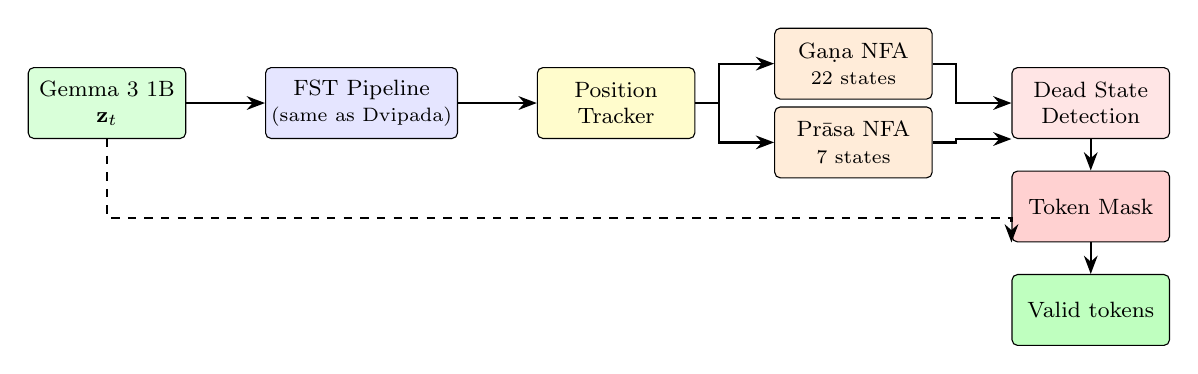
\begin{tikzpicture}[
  node distance=4mm and 8mm,
  box/.style={rectangle, draw, rounded corners=2pt, fill=blue!10,
              minimum width=20mm, minimum height=9mm,
              font=\footnotesize, align=center, inner sep=2pt},
  nfa/.style={rectangle, draw, rounded corners=2pt, fill=orange!15,
              minimum width=20mm, minimum height=9mm,
              font=\footnotesize, align=center, inner sep=2pt},
  >=Stealth
]
\node[box, fill=green!15] (llm) {Gemma 3 1B\\$\mathbf{z}_t$};
\node[box, right=10mm of llm] (fst) {FST Pipeline\\{\scriptsize (same as Dvipada)}};
\node[box, fill=yellow!20, right=10mm of fst] (pt) {Position\\Tracker};
\node[nfa, right=10mm of pt, yshift=5mm] (gn) {Ga\d{n}a NFA\\{\scriptsize 22 states}};
\node[nfa, right=10mm of pt, yshift=-5mm] (pn) {Pr\=asa NFA\\{\scriptsize 7 states}};
\node[box, fill=red!10, right=10mm of gn, yshift=-5mm] (dead) {Dead State\\Detection};
\node[box, fill=red!18, below=4mm of dead] (mask) {Token Mask};
\node[box, fill=green!25, below=4mm of mask] (out) {Valid tokens};
\draw[->, thick] (llm) -- (fst);
\draw[->, thick] (fst) -- (pt);
\draw[->, thick] (pt.east) -- ++(3mm,0) |- (gn.west);
\draw[->, thick] (pt.east) -- ++(3mm,0) |- (pn.west);
\draw[->, thick] (gn.east) -- ++(3mm,0) |- (dead.west);
\draw[->, thick] (pn.east) -- ++(3mm,0) |- (dead.south west);
\draw[->, thick] (dead) -- (mask);
\draw[->, thick] (mask) -- (out);
\draw[->, dashed, thick] (llm.south) -- ++(0,-10mm) -| (mask.south west);
\end{tikzpicture}%
}
\caption{Ragale Symbolic Enforcer. Compared to the Dvipada pipeline
(Figure~\ref{fig:enforcer}), Yati NFA is removed and the Ga\d{n}a NFA
uses 22 states (2 patterns) instead of 69 (8 patterns). The FST pipeline
is identical except for Kannada Unicode codepoints.}
\label{fig:ragale_enforcer}
\end{figure}

% -------------------------------------------------------------------------
\section{Generation Examples}
\label{app:examples}
% -------------------------------------------------------------------------

This appendix presents paired success and failure examples for the
five most important cells of Tables~\ref{tab:dvipada-results}
and~\ref{tab:ragale-results}, plus the adapted Chandomitra baseline.
Each example shows the generated couplet in RTS romanisation
(matching the prompt convention of Section~\ref{sec:evaluation}), the
FST-emitted U/I (\textit{guru}/\textit{laghu}) syllable-weight markers,
and a per-constraint verdict ($\checkmark$~= pass, $\times$~= fail).
Examples are selected deterministically as the lowest seed satisfying
the filter (all-valid for successes, not-all-valid for failures); cells
that are 100\% valid use the lowest-seed record. Original Telugu and
Kannada script for every example is available in the corresponding
benchmark JSON file.

\subsection{Dvipada (Telugu)}
\label{app:examples_dvipada}

\paragraph{Hybrid, gemma3-1b-merged --- success.}
Topic: \textit{tallI prEma annintikaMTe goppadi} (mother's love).

\begin{quote}
\textit{liMgamaMtayu niMpeDi briyamu liMga} \\
\textit{liMgaMbunaMduna nellavArikini} \\
\textsc{U/I L1:} U I U I I U I I I I I U I \\
\textsc{U/I L2:} U U I U I I U I U I I I \\
\textbf{Verdict:} \textit{ga\d{n}a} $\checkmark$,
\textit{pr\={a}sa} $\checkmark$, \textit{yati} $\checkmark$
\\ {\footnotesize seed=42, backtracks=0, tokens=35, elapsed=2.04\,s}
\end{quote}

\paragraph{Masking-only, gemma3-1b-base --- success.}
Topic: \textit{tallI prEma annintikaMTe goppadi}. The base model
collapses onto a degenerate but technically valid loop, repeating the
same line verbatim --- still passes all three constraints.

\begin{quote}
\textit{nati nUta nUta nUta nanUnakaina} \\
\textit{nati nUta nUta nUta nanUnakaina} \\
\textsc{U/I L1:} I I U I U I U I I U I U I \\
\textsc{U/I L2:} (identical to L1) \\
\textbf{Verdict:} \textit{ga\d{n}a} $\checkmark$,
\textit{pr\={a}sa} $\checkmark$, \textit{yati} $\checkmark$
\\ {\footnotesize seed=42, backtracks=0, tokens=36, elapsed=2.70\,s}
\end{quote}

\paragraph{Masking-only, gemma3-1b-base --- failure.}
Topic: \textit{SrIrAmuDu sItAdEvini rakshiMcuTaku laMkaku veLLenu}
(Rama goes to Lanka). Line~1's foot partition is valid, but line~2
admits no legal Indra$^3$\,$\cdot$\,Surya partition over its 11
emitted syllables.

\begin{quote}
\textit{nalakala naMdena nalakala naMda} \\
\textit{sIlakunaMdena sItAmatini} \\
\textsc{U/I L1:} I I I I U I I I I I I U I \\
\textsc{U/I L2:} U I I U I I U U I I I \\
\textbf{Verdict:} L1 \textit{ga\d{n}a} $\checkmark$;
L2 \textit{ga\d{n}a} $\times$
(no valid foot partition).
\\ {\footnotesize seed=42, backtracks=0, tokens=42, elapsed=2.80\,s}
\end{quote}

\subsection{Ragale (Kannada)}
\label{app:examples_ragale}

\paragraph{Hybrid, gemma3-1b-lora --- success.}
Topic: \textit{Bubbles}. Both lines reach the canonical
$\text{III}^3 \cdot \text{IIU}$ partition with the structurally
required \textit{guru} ending.

\begin{quote}
\textit{kanasu muDiyu kadana hasivA} \\
\textit{olavanu kaDalanu madhuravA} \\
\textsc{U/I L1:} I I I I I I I I I I I U \\
\textsc{U/I L2:} I I I I I I I I I I I U \\
\textbf{Verdict:} \textit{ga\d{n}a} $\checkmark$
($\text{III}\,\text{III}\,\text{III}\,\text{IIU}$),
\textit{pr\={a}sa} $\checkmark$, \textit{guru}-ending $\checkmark$
\\ {\footnotesize seed=42, backtracks=0, tokens=27, elapsed=2.64\,s}
\end{quote}

\paragraph{Masking-only, gemma3-1b-base --- failure.}
Topic: \textit{Bubbles}. Line~1 emits only 10 syllables (the metre
requires exactly 12) and does not end on \textit{guru}; line~2 happens
to recover the canonical pattern. This illustrates the dominant
Ragale-base failure mode: stateless masking lets the model
under-shoot the line target.

\begin{quote}
\textit{ba cilA asakana as padya} \\
\textit{gaNanakana karaka karaka nE} \\
\textsc{U/I L1:} I I U I I I I U U I \quad (10 syllables) \\
\textsc{U/I L2:} I I I I I I I I I I I U \quad (12 syllables) \\
\textbf{Verdict:} L1 \textit{ga\d{n}a} $\times$ (10 syllables, expected 12),
\textit{guru}-ending $\times$;
L2 \textit{ga\d{n}a} $\checkmark$.
\\ {\footnotesize seed=42, backtracks=0, tokens=65, elapsed=9.81\,s}
\end{quote}

\subsection{Adapted Chandomitra Baseline}
\label{app:examples_chandomitra}

\paragraph{Chandomitra, gemma3-1b-merged --- rare success.}
Topic: \textit{hanumaMtuDu samudramunu dATi laMkanu cErenu}
(Hanuman crosses to Lanka). One of only 14 valid records out of 102.

\begin{quote}
\textit{saraLamaina va bhASa jUpakuMDa livi} \\
\textit{baraga nanilajayapratimapadmamula} \\
\textbf{Verdict:} \textit{ga\d{n}a} $\checkmark$,
\textit{pr\={a}sa} $\checkmark$, \textit{yati} $\checkmark$
(per-constraint scores 100/100/100 from the chandomitra
\texttt{breakdown} field).
\\ {\footnotesize seed=49, backtracks=0, tokens=28, elapsed=0.64\,s}
\end{quote}

\paragraph{Chandomitra, gemma3-1b-merged --- failure.}
Topic: \textit{tallI prEma annintikaMTe goppadi}. The most common
adapted-Chandomitra failure mode: the model never emits a line break
and the top-$k$ filter exhausts the 150-token budget on a single
runaway line. This is the structural dead-state issue described in
the §10 \emph{Comparison to Chandomitra} paragraph.

\begin{quote}
\textit{saraLamaina vArakulu nirmANaMDabhuvaMTi vyeMDEgodhikaNa
pramukhacE pada\-vaMta ravidya cakra SiSEcElaM~\ldots}
[150 tokens, no newline, no valid couplet emitted]
\\
\textbf{Verdict:} L1 \textit{ga\d{n}a} $\times$ (no foot partition over
the runaway syllable stream); L2 \textbf{never emitted}.
\\ {\footnotesize seed=42, backtracks=0, tokens=150, elapsed=104.35\,s}
\end{quote}

\paragraph{Chandomitra, gemma3-1b-base --- failure.}
Topic: \textit{tallI prEma annintikaMTe goppadi}. A pedagogically
useful failure: \textit{ga\d{n}a} passes on both lines, but
\textit{pr\={a}sa} fails (the second-syllable consonants
$m$ and $r$ are not in the same equivalence group) and \textit{yati}
fails on line~1 (foot~1 first letter and foot~3 first letter belong
to different \textit{maitri} groups).

\begin{quote}
\textit{ammA dayakulE toli saha kar vyara Ta} \\
\textit{pada prativara mUDu mahavaccu lakSa} \\
\textbf{Verdict:} \textit{ga\d{n}a} $\checkmark/\checkmark$,
\textit{pr\={a}sa} $\times$ ($m \not\equiv r$),
\textit{yati} $\times/\checkmark$ (L1 fails, L2 passes; aggregate
yati score 50/100 in the chandomitra \texttt{breakdown}).
\\ {\footnotesize seed=42, backtracks=0, tokens=23, elapsed=2.31\,s}
\end{quote}

\end{document}
